\section{Study of the Monte Carlo cocktail production}
The second part of the analysis of this thesis is devoted to the study of \textbf{Belle II Monte Carlo cocktail simulations}. A Belle II "cocktail" MC production (typically generated with Pythia8) simulates all relevant physics channels simultaneously. Therefore, the analyzed channel $e^+e^- \rightarrow p\pi^-\bar{n}\,(\gamma_\text{ISR})$ is now embedded within all other background channels in the cocktail; the first task is to correctly reconstruct it amidst the surrounding backgrounds, studying the recoil mass distribution.
$\\$
To achieve this, a first attempt uses the complete RUN1 $u\bar{u}$ production. Building on the signal sample discussed in the last chapter, further optimal cuts and selection criteria are developed to properly isolate the signal in the recoil mass distribution. Therefore the corresponding shower shape variables of neutral cluster associated to anti-neutron candidates are studied.
$\\$
Eventually, the full Belle II $q\bar{q}$ ($u\bar{u}$, $d\bar{d}$, $c\bar{c}$, $s\bar{s}$) production is analyzed. The resulting cluster variables are compared with those from real data to assess Data/MC agreement.

\begin{figure}[H]
    \centering
    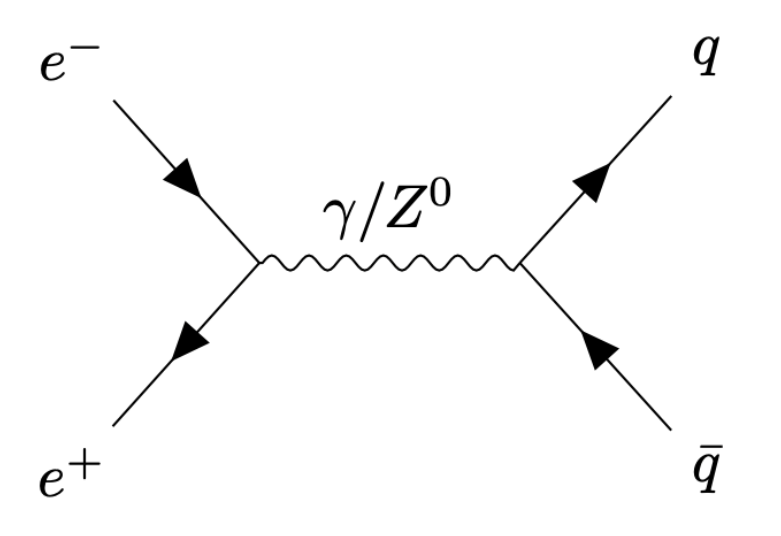
\includegraphics[width=0.45\textwidth]{nbar_cocktail/images/qqbar_diag}
    \caption{Tree level Feynman diagram of $e^+ e^- \to q \bar{q}$}
\end{figure}
First of all, it could be useful start describing the Belle II Distributed Computing, namely the Belle II Grid.

\subsection{Introduction to the Belle II Distributed Computing}
Belle II datasets are categorized into two main types: \textbf{Data} and \textbf{Monte Carlo}. The Data are obtained from calibrated collision events processed by the experiment. Monte Carlo samples are generated using the Monte Carlo method according to various event generators, as discussed in Chapter 2. These are further classified into \textbf{Signal MC}- a specific process generated with a dedicated decay file upon analyst request (as in the previous chapter)- and \textbf{Generic MC}, or "cocktail'', containing all processes expected in data with their correct relative fractions (as in the present chapter). These are usually in mdst (Mini Data Summary Table) format. There is cdst (Calibration Data Summary Table) as well, but it is used mainly to address calibration tasks.
$\\$
Data and Monte Carlo samples can be ``skimmed'' by applying analysis-dependent offline pre-selections called ``skims''. Skims reduce data volume by selecting events of interest for specific analyses and retaining only the necessary information, producing smaller, more manageable datasets.
$\\$
Using these Data and MC collections, analyses are performed via custom steering files with basf2, producing final ROOT ntuples. Subsequent offline analysis is then conducted outside the basf2 framework using ROOT, matplotlib, etc.
$\\$
A scheme of the Belle II Data Model is shown below:

\begin{figure}[H]
    \centering
    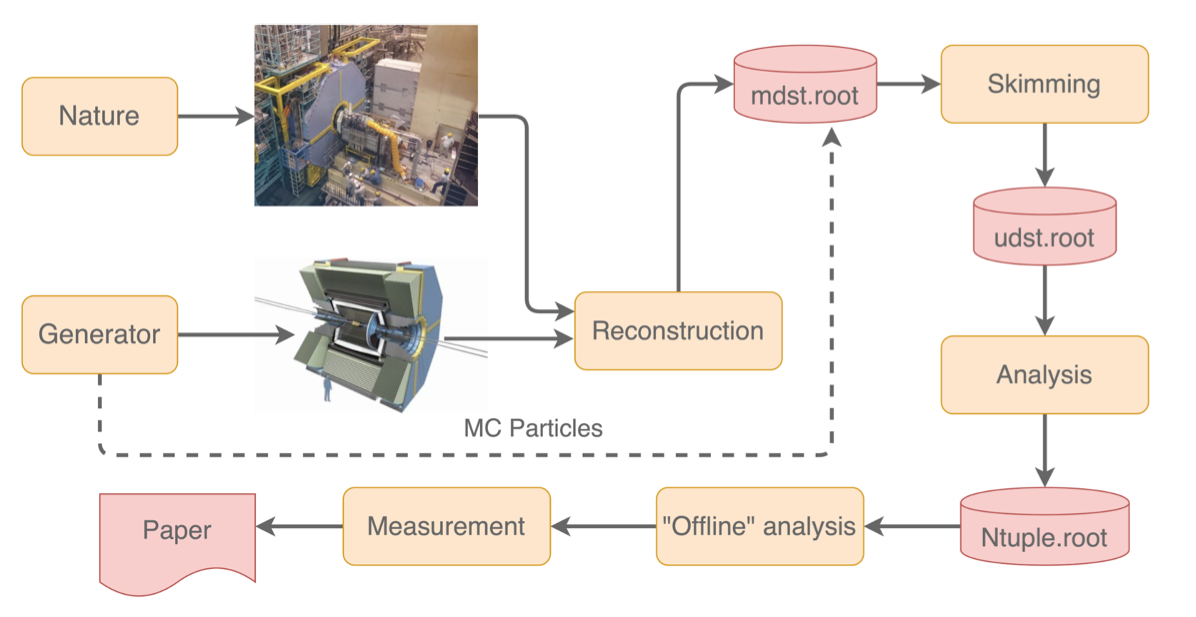
\includegraphics[width=1\textwidth]{nbar_cocktail/images/datafiles}
    \caption{A scheme of the Belle II Data Model, starting from the nature processes information to the final results. As described, Monte Carlo truth information bypasses reconstruction, since the information is directly picked at generator level}
\end{figure}

Belle II Data and Monte Carlo samples are distributed across numerous storage sites worldwide. This Distributed Computing System, known as \textbf{the Grid}, consists of a network of loosely coupled computers with varying local conditions (operating systems, resources, etc.). 
$\\$
Two full copies of the raw data are maintained at dedicated data centers. Raw data is processed, skimmed, and distributed over other storage sites:

\begin{figure}[H]
    \centering
    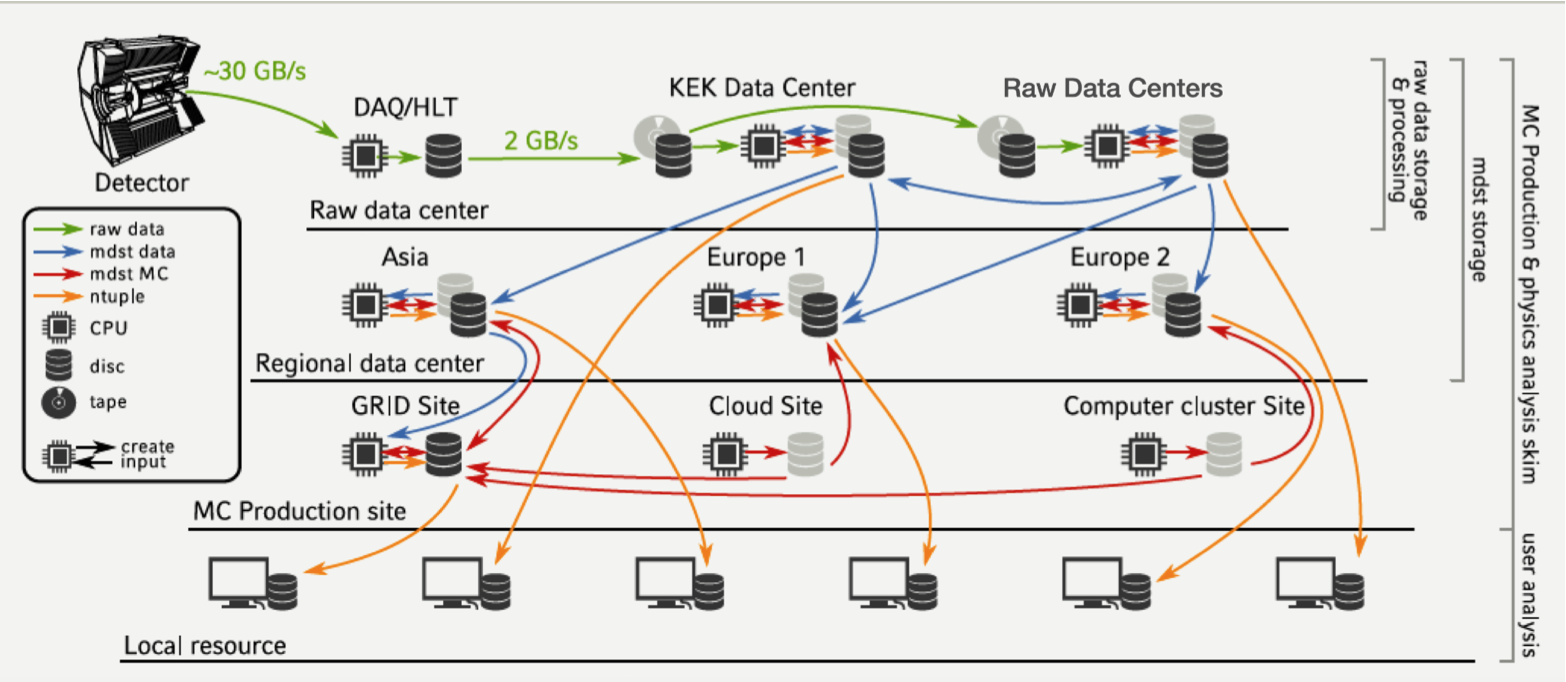
\includegraphics[width=1\textwidth]{nbar_cocktail/images/grid_distribution}
    \caption{A scheme of the Belle II Distributed Computing (The Grid) sites }
\end{figure}

Each site interact with \textbf{DIRAC}, an interware that manages interactions between Belle II and its computing resources. \textbf{BelleDIRAC} is an extension that enables users to interact with DIRAC for job submission, data placement, monitoring, and other tasks.

\subsubsection{Types of processes at the Belle experiment enviroment}
Many processes can occur during an $e^+e^-$ collision. These may mimic the selected signal and be accidentally reconstructed as signal events, though they represent background processes.
$\\$
The types of processes present depend on if beams collide on-resonance or off-resonance in reference to the $\Upsilon(4S)$ resonance. $\Upsilon(4S)$ production occurs at $\sqrt{s} = 10.58$ GeV, yielding 
$\Upsilon(4S) \rightarrow BB$ processes. The $B^+B^-$ and $B^0 \bar{B}^0$ final states  are referred to as charged and neutral $B \bar{B}$ pairs, respectively.
$\\$
$e^+e^- \to q\bar{q}$ ($q = u,d,s,c$) processes, known as continuum production, also occur. The production cross section of the Belle II processes is shown below:

\begin{table}[h]
\centering
\begin{tabular}{l r}
Process & Cross section (nb) \\
$e^+e^- \to \Upsilon(4S)$ & 1.10 \\
$e^+e^- \to u\bar{u} (\gamma)$ & 1.61 \\
$e^+e^- \to d\bar{d} (\gamma)$ & 0.40 \\
$e^+e^- \to s\bar{s} (\gamma)$ & 0.38 \\
$e^+e^- \to c\bar{c} (\gamma)$ & 1.30 \\
$e^+e^- \to \tau^+\tau^- (\gamma)$ & 0.92 \\
$e^+e^- \to e^+e^- (\gamma)$ & 300 \\
$e^+e^- \to \mu^+\mu^- (\gamma)$ & 1.15 \\
$e^+e^- \to \gamma \gamma (\gamma)$ & 4.99 \\
$e^+e^- \to e^+e^-e^+e^-$ & 39.7 \\
$e^+e^- \to e^+e^-\mu^+\mu^-$ & 18.9 \\
\end{tabular}
\end{table}

\begin{figure}[H]
    \centering
    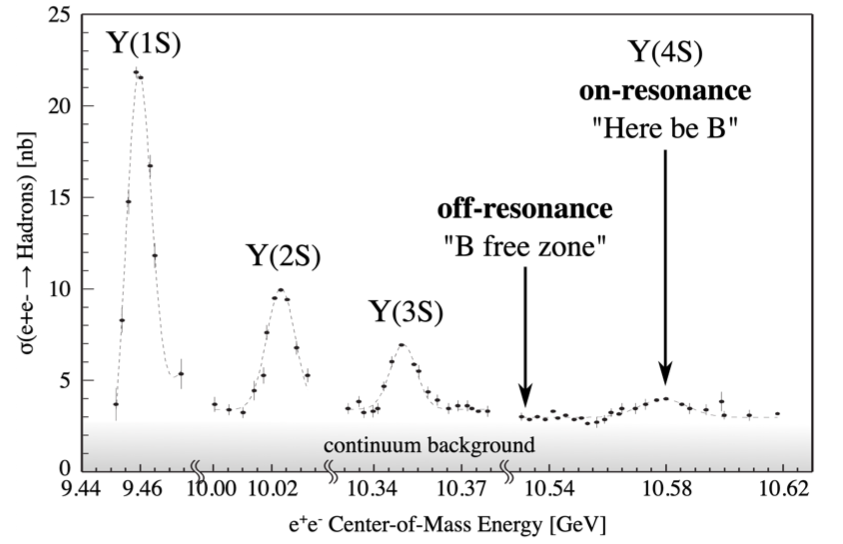
\includegraphics[width=0.75\textwidth]{nbar_cocktail/images/BelleII_processes}
    \caption{Cross section of $e^+ e^- \rightarrow Hadrons$, in $\Upsilon$ resonances energy region \cite{BelleIIPhysicsBook2019}. $\Upsilon(1S)$ resonance is very narrow, while $\Upsilon(4S)$ one is broader and lower}
\end{figure}

\subsection{Applied selections and cuts}
To follow the same approach as used in the signal sample analysis, the recoil mass is first studied using the complete $u\bar{u}$ cocktail production, which corresponds to a $\sim 1429.23 \ fb^{-1}$ integrated luminosity of data.
$\\$
The following real cuts have been applied:
\begin{enumerate}
\item Recoil system: $0 \ GeV/c^2 <recoil \ mass < 2 \ GeV/c^2$
\item $\bar{n}$: neutral clusters from ECL and number of hits $> 10$ and energy $<3$ GeV
\item $p$: $protonID > 0.9$ and $dr<1$ cm and $|dz|<3$ cm 
\item $\pi^-$: $pionID > 0.1$ and $dr<1$ cm and $|dz|<3$ cm 
\item $\alpha <0.20$ rad $\sim 11.5 ^{\circ}$
\item No further charged particles in the Rest of Event (ROE)
\end{enumerate}

Four additional cuts are applied beyond those used for the signal sample, such as cluster number of hits $> 10$ GeV, $\alpha <0.20$ rad, the request of no further charged particles in the Rest of Event (ROE) and the energy of the neutral cluster associated to $\bar{n}$ candidates must be less then 3 GeV.
$\\$
The first cut arises from observations in the previous chapter; to achieve cleaner selection of neutral clusters associated with anti-neutron candidates -reducing cluster split-off and pre-showering contributes- a requirement on the number of lighted crystals is applied. 
$\\$
The second cut allows a stricter selection of anti-neutron candidates through a smaller $\alpha$ angle. $\alpha$ is defined as the 3D angle between the recoil vector and the neutral cluster associated with the $\bar{n}$. As will be explained later, this threshold will be lowered further.
$\\$
To explain the third cut, the concept of \textbf{Rest of Event} (ROE) must first be introduced. The ROE is built around the reconstructed target particles and consists of all other particles in the rest of event. In the present case, the reconstructed particles are $p, \pi^-, \bar{n}$ (and $\gamma_{ISR}$); therefore, the ROE includes all particles outside this reconstructed system. Consequently, the third selection criterion requires that no charged particles (i.e. tracks associated with charged particles) be present in the Rest Of Event, providing a cleaner event reconstruction. 

\begin{figure}[H]
    \centering
    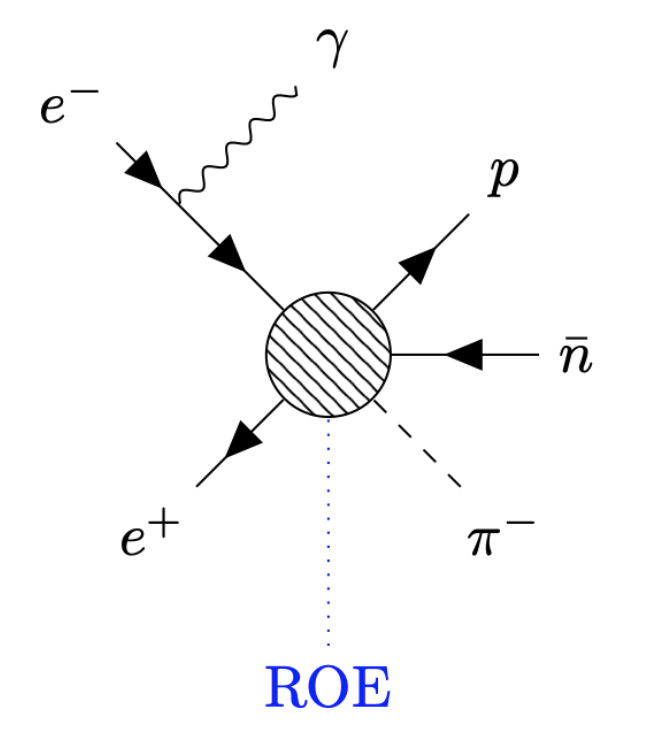
\includegraphics[width=0.45\textwidth]{nbar_cocktail/images/ROE_diag}
    \caption{The selected channel with ROE made of a variable amount of particles.}
\end{figure}

The fourth cut arises from cluster energy studies performed on the first chunk of $u\bar{u}$ cocktail production, corresponding to $\sim 215 fb^{-1}$. The $\bar{n}$ list can be affected by several mis-identified $\gamma_\text{ISR}$. In order to study this phenomenon, the Monte Carlo ISR flag (mcISR) can be used to separate the two contributions in reconstructed $\bar{n}$ list. mcISR variable is a Monte Carlo flag; If mcISR = 0, the reconstructed particle is not an ISR photon. If mcISR = 1, the reconstructed particle is an ISR photon mis-identified as an anti-neutron. The obtained cluster energy distribution for $\bar{n}$ candidates is shown in figure ~\ref{fig:E_isr}.
$\\$
It is easy to note that two structures at $\sim 4$ GeV and $\sim 6$ GeV, due to $\gamma_{ISR}$ mis-identified as anti-neutrons, arise. In order to remove them, a cut on cluster energy such as those applied is mandatory.
\begin{figure}[h]
    \centering
    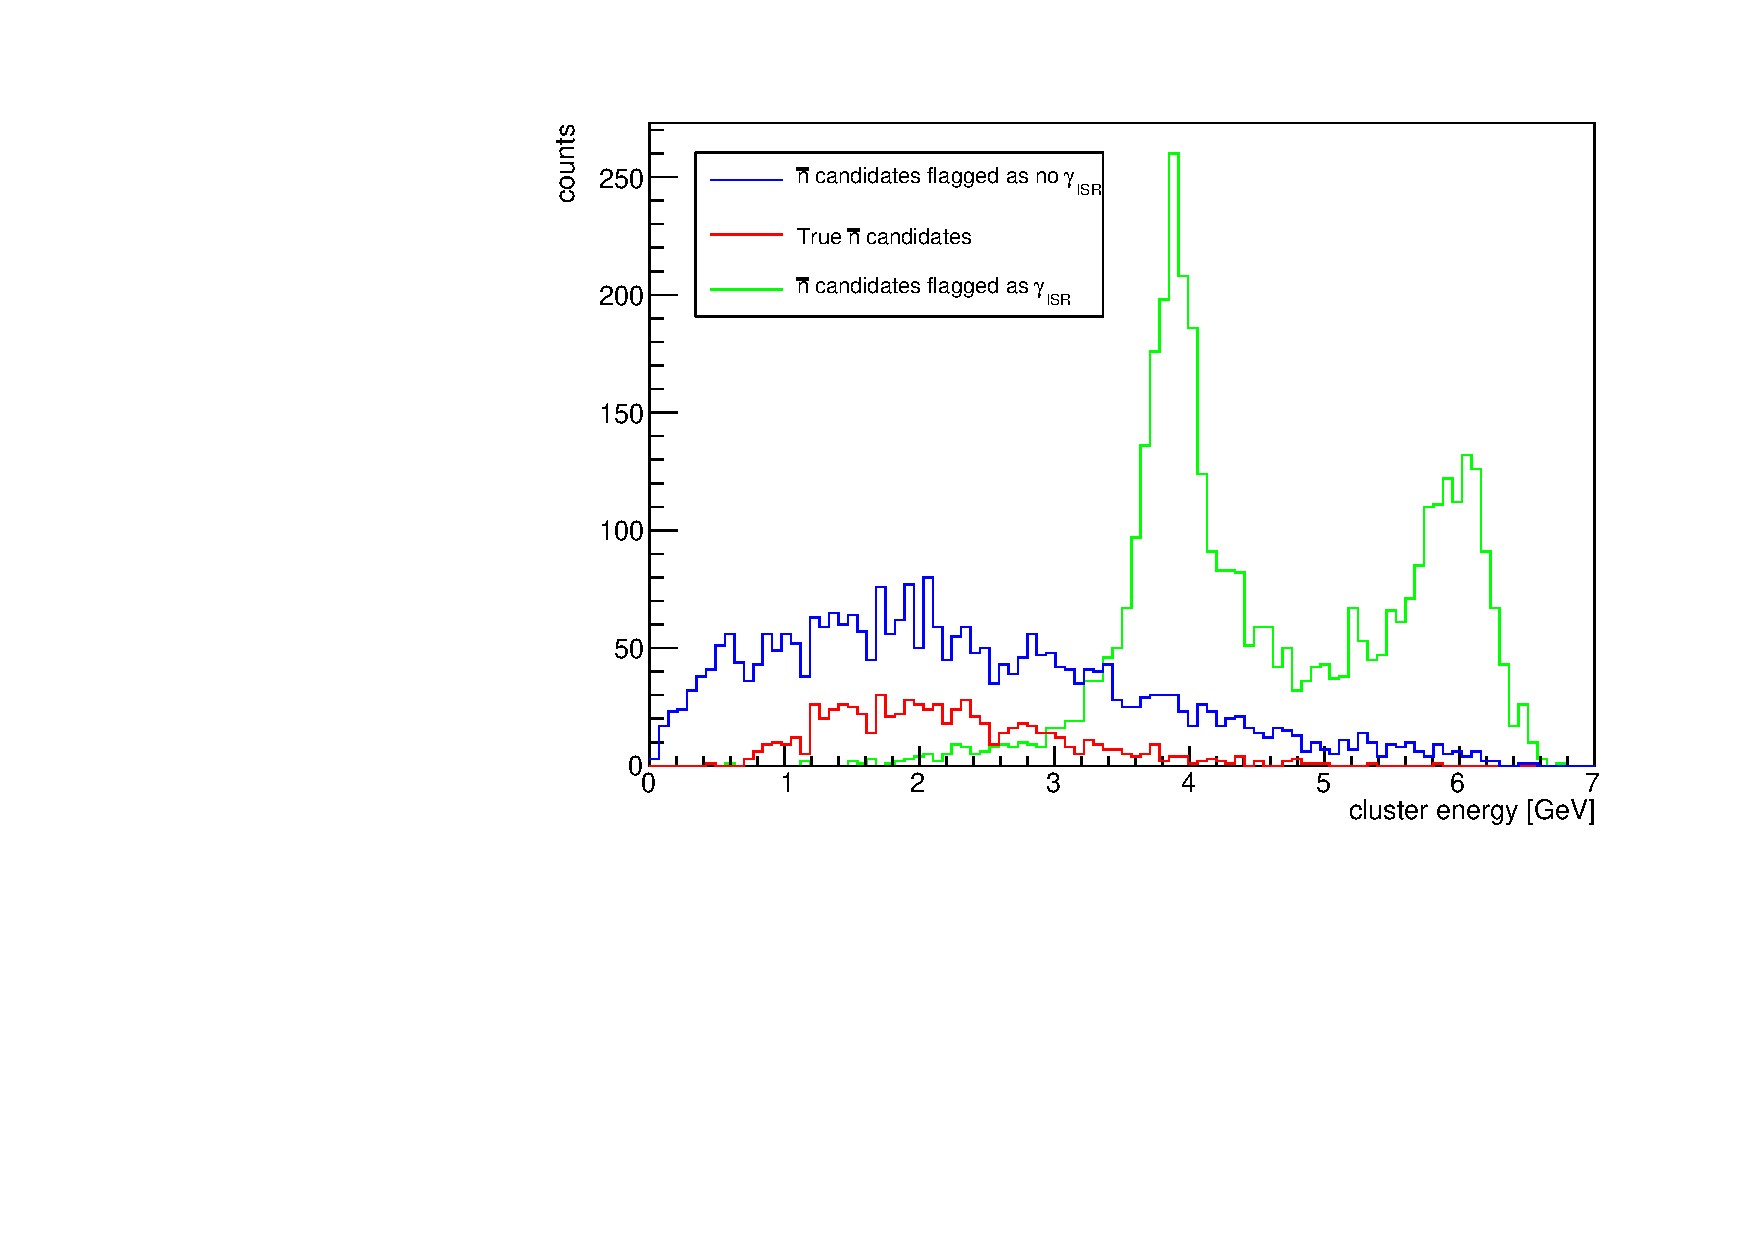
\includegraphics[width=0.80\textwidth]{nbar_cocktail/images/clusterEnergy_isr}
    \caption{Cluster energy distribution of $\bar{n}$ candidates, divided by the Monte Carlo ISR flag (\texttt{mcISR}). If \texttt{mcISR} = 0, the reconstructed particle is not an ISR photon. If \texttt{mcISR} = 1, the reconstructed particle is an ISR photon. Of course this is a level-generator information.}
    \label{fig:E_isr}
\end{figure}
$\\$
However, $\gamma$ radiation represents one of the most abundant produced particles in HEP experiments such as Belle II, making a major contribution to the background. In addition to the ISR ($E \sim 10$ MeV - $5$ GeV) and FSR ($E< 10$ MeV) radiation described above, bremsstrahlung ($E < 50$ MeV) and secondary photons -such as those from $\pi^0 \rightarrow \gamma \gamma$ decays  ($E < 400$ MeV)- are also present. Therefore, NO ISR channel where the recoil system is made of  $p, \pi^-$ should represents a cleaner system to reconstruct than the ISR one where the recoil system is made of  $p, \pi^-, \gamma$, since several background $\gamma$'s can be mis-identified as the ISR photon, which must be accounted for in the recoil system.
$\\$
In order to compare the feasibility of selecting the channel in both ISR and NO ISR cases separately, the recoil mass distribution must be first studied using the same selection criteria. The better the selection of the signal from the background, the more consistent the shower shape variables will be for neutral clusters associated with $\bar{n}$ candidates, eventually allowing proper Data/MC agreement for these variables.

\subsection{Recoil mass in $u\bar{u}$ cocktail production (NO ISR case)}
The recoil mass distribution obtained from the $u\bar{u}$ cocktail is first studied in NO ISR case. If the recoil system $p, \pi^-$ is properly reconstructed among all possible background channels, then a peak should be observed at the anti-neutron rest mass ($939.5$~MeV/$c^2$). The obtained result is shown in ~\ref{fig:mRec_nog_020}.
\begin{figure}[h]
    \centering
    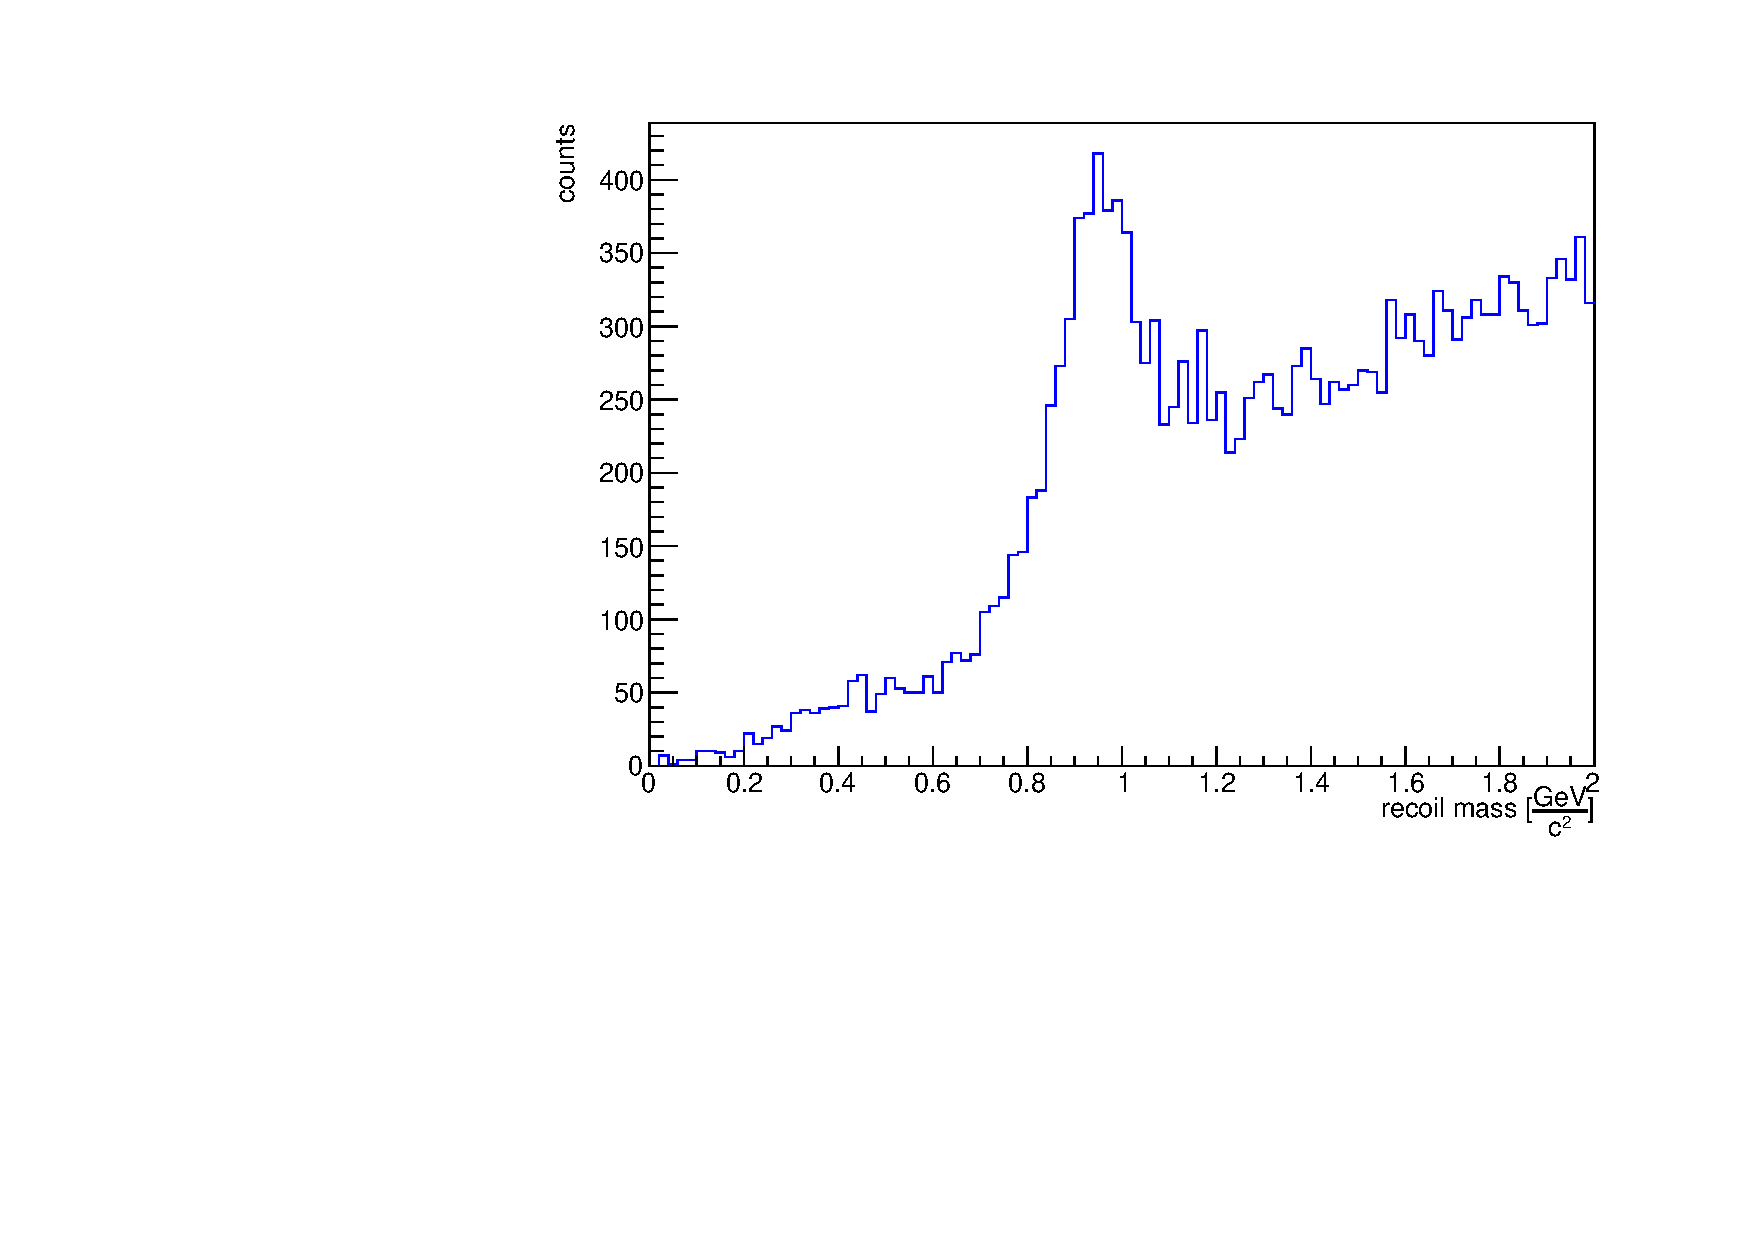
\includegraphics[width=0.80\textwidth]{nbar_cocktail/images/recoil_mass_nog_020}
    \caption{Reconstructed $p, \pi^-$ recoil mass distribution in $u\bar{u}$ Monte Carlo cocktail, NO ISR case.}
    \label{fig:mRec_nog_020}
\end{figure}

A distinct structure is observed above the $\bar{n}$ mass value, suggesting that the selected channel is properly reconstructed. For a cleaner comparison between the signal channel and background components, the TopoAna output can be consulted ~\ref{fig:topo_nog_020}. TopoAna does not account for particle-matter interactions; thus, all displayed particles originate directly from the $e^+e^-$ collision at the IP.
\begin{figure}[H]
    \centering
    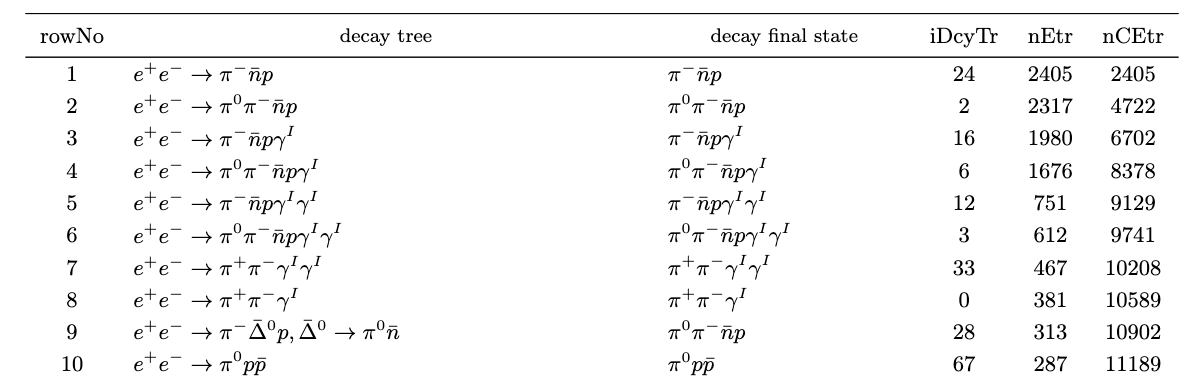
\includegraphics[width=1\textwidth]{nbar_cocktail/images/topoana_nog_020}
    \caption{First 10 channels of the TopoAna output in $u\bar{u}$ Monte Carlo cocktail, showing the different channel contributes, NO ISR case.}
    \label{fig:topo_nog_020}
\end{figure}

Accessing the Monte Carlo information from TopoAna, it is clear that the main contribution comes from the signal channel with $p \pi^- \bar{n}$ in the final state, immediately followed by the one with $p \pi^- \bar{n} \pi^0$ in the final state. Further contribution arise from $p \pi^- \bar{n} \gamma_{ISR}$, which could be interpreted as signal, even if, in NO ISR case, the $\gamma_{ISR}$ is not explicitly reconstructed within the recoil system. The fourth contribute is due to the one with $p \pi^- \bar{n} \pi^0 \gamma_{ISR}$ and so on. It is important to note that the contributions are sorted from most to least abundant.

\subsubsection{Recoil mass components analysis}
The recoil mass distribution components can be studied by correlating the ntuple information obtained from the steering file with that produced by the TopoAna program. 
$\\$
Each channel is identified by its own \texttt{iDcyTr} (index of the decay tree), which allows one to represent the contribution of a given channel (or a combination of channels) to a specific variable, such as the recoil mass of the system $p \pi^-$.
$\\$
The components are therefore denoted as follows:
\begin{enumerate}
\item $e^+ e^- \rightarrow \pi^- \bar{n} p$ (iDcyTr == 24)
\item $e^+ e^- \rightarrow \pi^0 \pi^- \bar{n} p$ (iDcyTr == 2)
\item $e^+ e^- \rightarrow \pi^- \bar{n} p \gamma_{ISR}$ (iDcyTr == 16)
\item $e^+ e^- \rightarrow \pi^0 \pi^- \bar{n} p \gamma_{ISR}$ (iDcyTr == 6)
\item $e^+ e^- \rightarrow$ other
\end{enumerate}
The obtained stacked component to the recoil mass are shown in figure ~\ref{fig:mRecComps_nog_020}.
\begin{figure}[h]
    \centering
    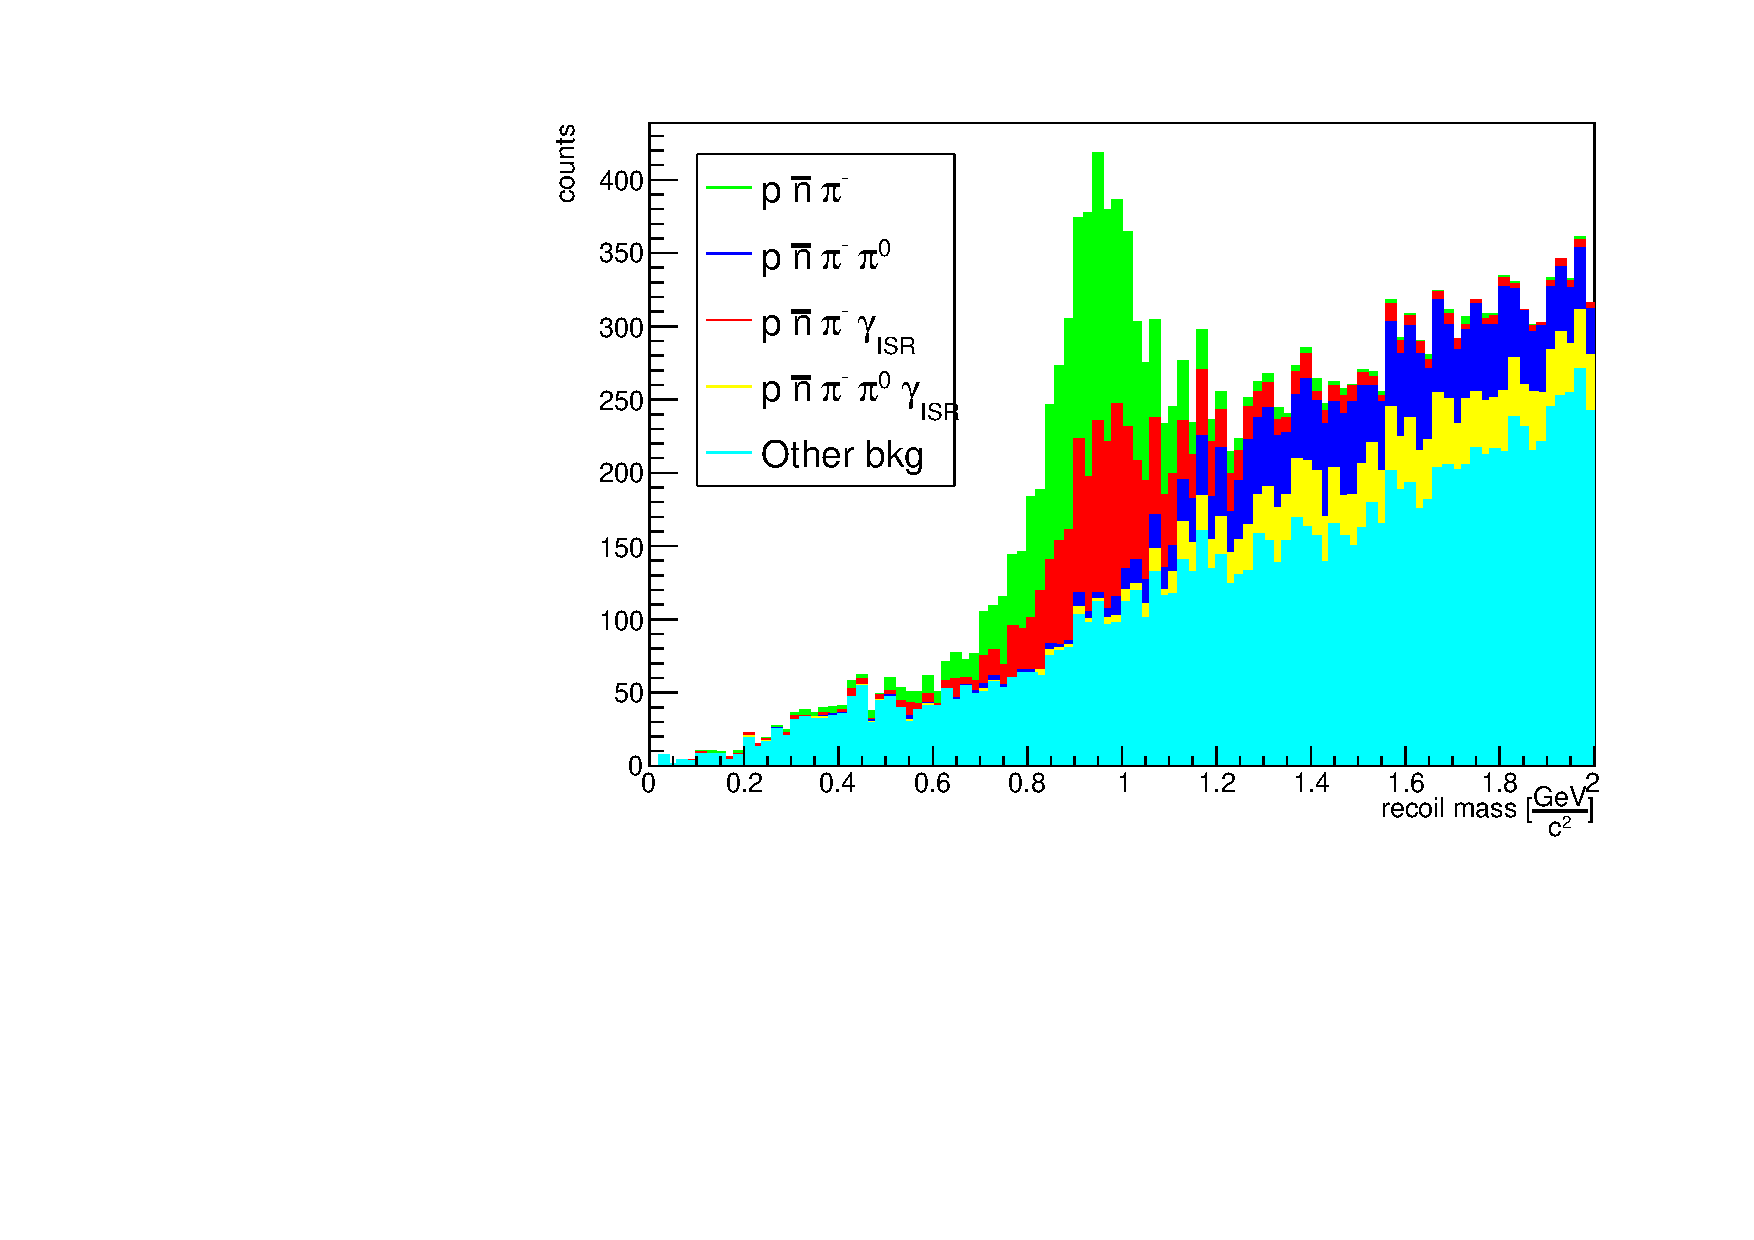
\includegraphics[width=0.90\textwidth]{nbar_cocktail/images/recoilM_comps_nog_020}
    \caption{$p, \pi^-$ recoil mass distribution in $u\bar{u}$ Monte Carlo cocktail, displaying each stacked component contribution, NO ISR case.}
    \label{fig:mRecComps_nog_020}
\end{figure}

Defining the \emph{Signal Region} as the interval $[0.8, 1.2]$ GeV, it can be observed that contributions from the channel with iDcyTr = 2 predominantly lie to the right of the signal region. This is expected, as the recoil system computation excludes the $\pi^0$. Same conclusion ca be made for the with iDcyTr = 6. 
$\\$
As expected, the signal channel (iDcyTr = 24) predominantly populates the signal region. The $\pi^- \bar{n} p \gamma_{ISR}$ channel (iDcyTr = 16) also mainly populates the signal region, indicating that the $\gamma_{ISR}$ is negligible and has minimal impact on the recoil mass, as shown by the ISR energy distribution in Fig.~\ref{fig:isr_distro}.
$\\$
This can be directly observed from the single contribute from these two channels displayed in figure ~\ref{fig:mRecComps_nog_020_0e3}.
\begin{figure}[H]
    \centering
    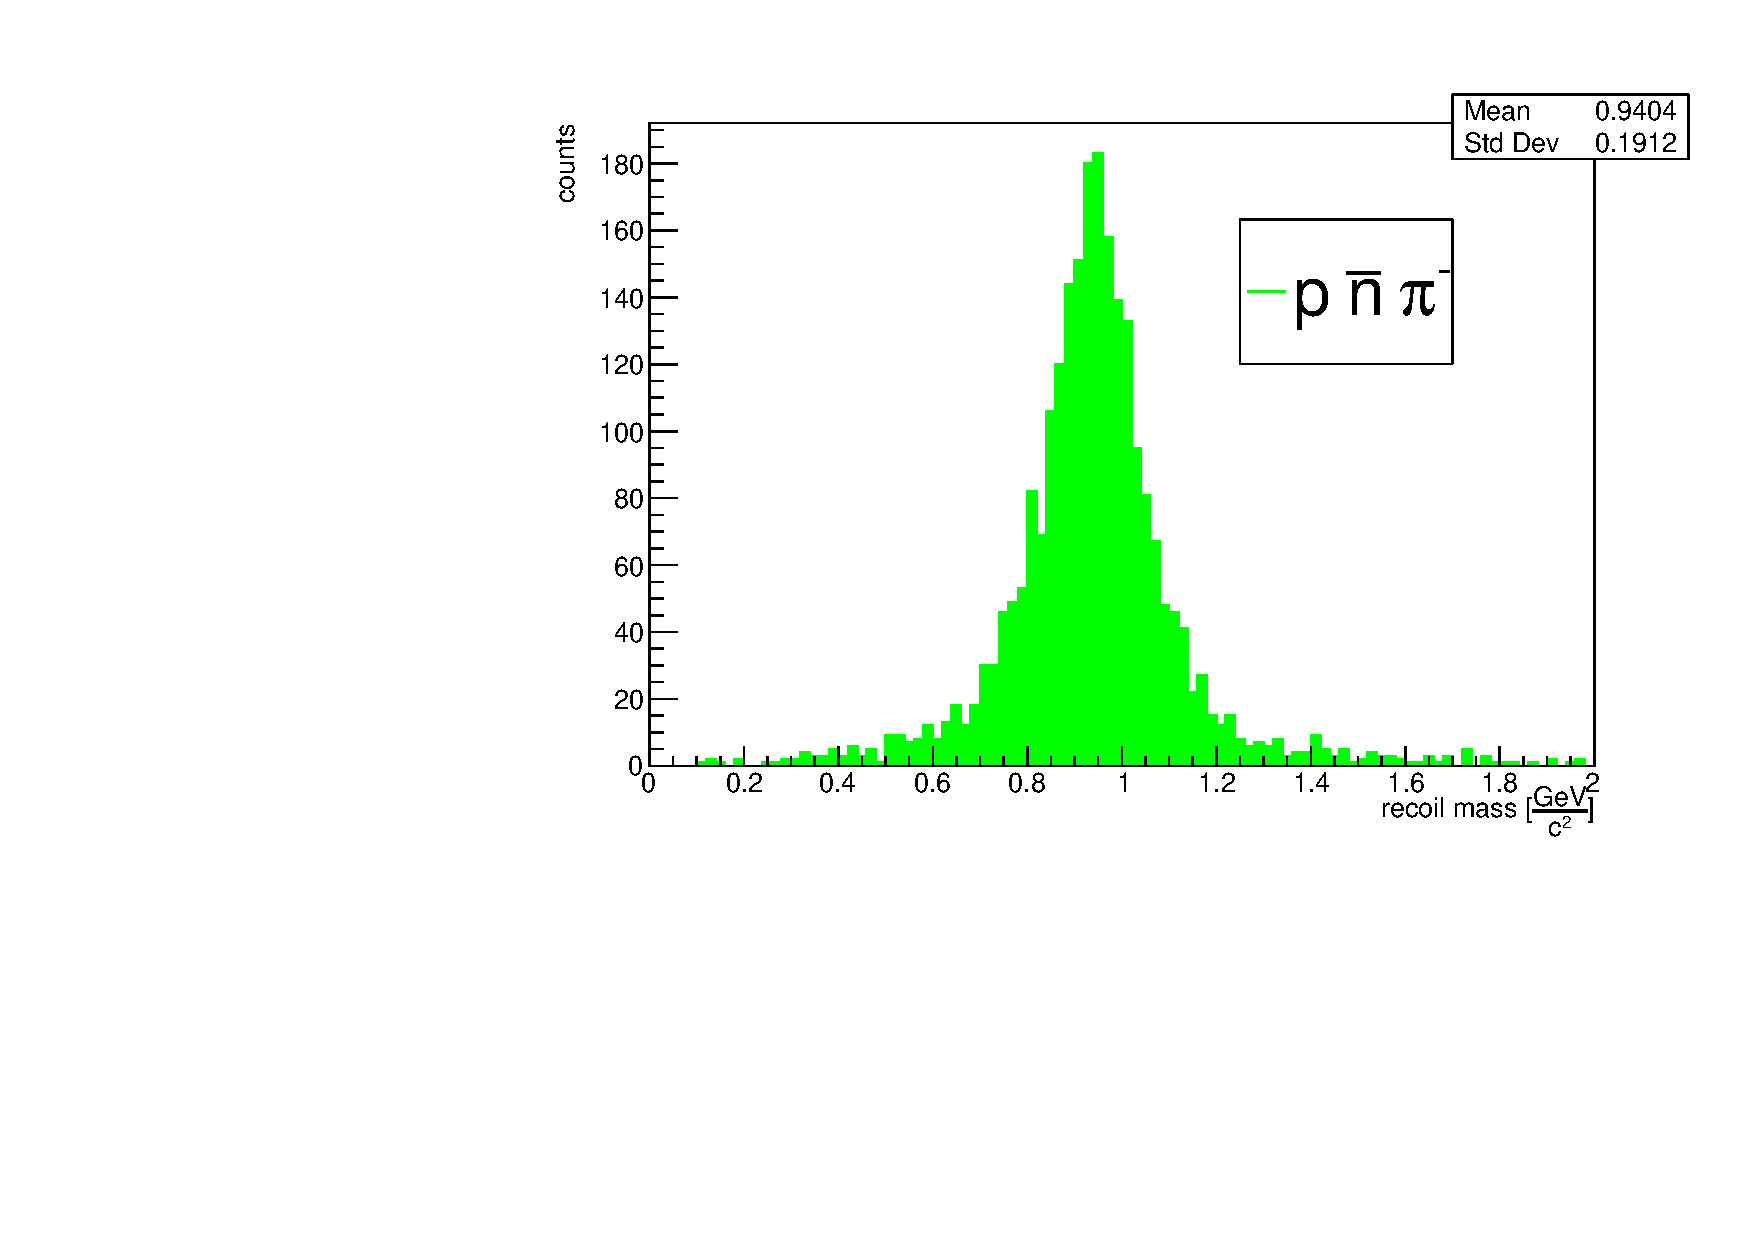
\includegraphics[width=0.49\textwidth]{nbar_cocktail/images/recoilM_comp0_nog_020}
    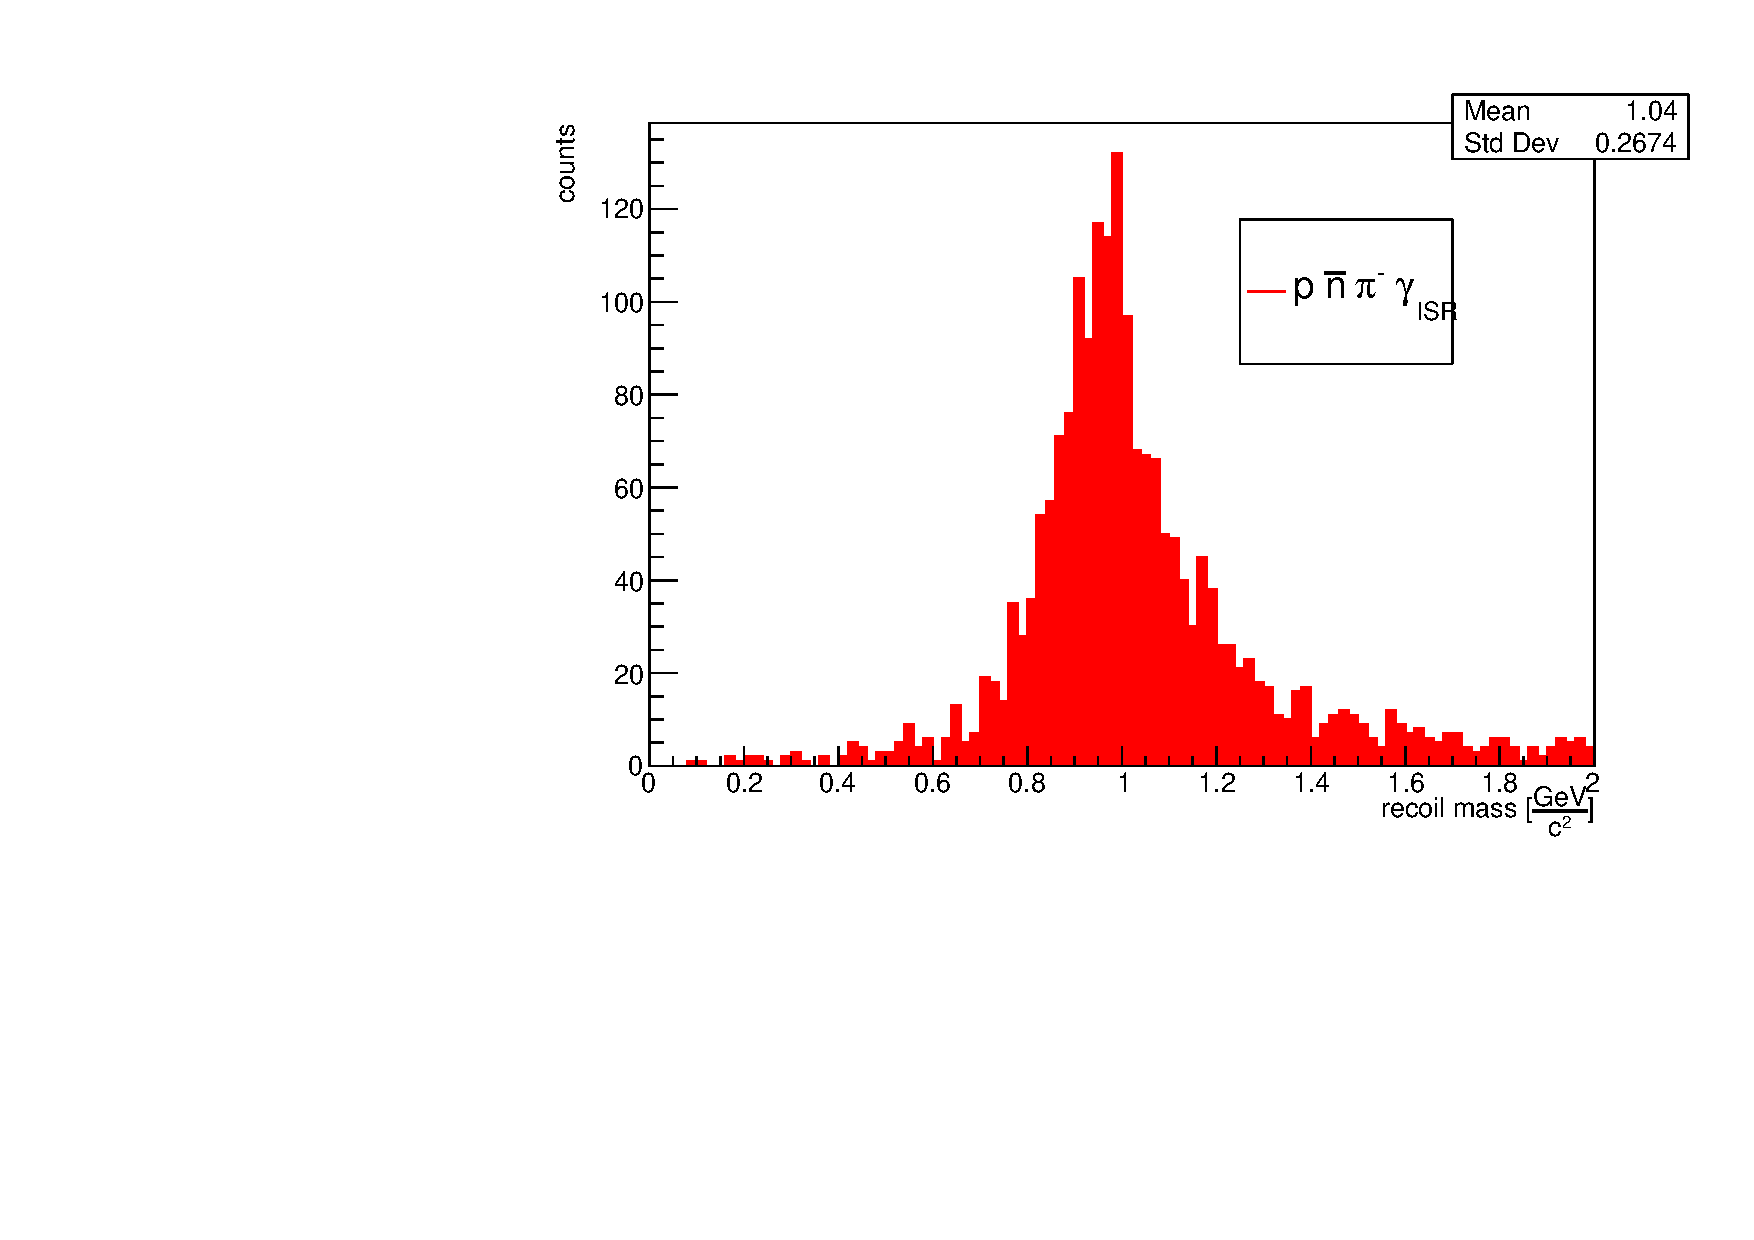
\includegraphics[width=0.49\textwidth]{nbar_cocktail/images/recoilM_comp3_nog_020}
    \caption{ (a) $p, \pi^-$ recoil mass and (b) $p, \pi^-, \gamma_{ISR}$ recoil mas distribution in $u\bar{u}$ Monte Carlo cocktail}
    \label{fig:mRecComps_nog_020_0e3}
\end{figure}
$\\$
Thus, despite the $\gamma_{ISR}$ not being directly reconstructed, the $\pi^- \bar{n} p \gamma_{ISR}$ channel (iDcyTr = 16) can be considered a signal channel. This leads to the recoil mass composition shown in figure .~\ref{fig:mRecComps_nog_020_0+3}.
\begin{figure}[h]
    \centering
    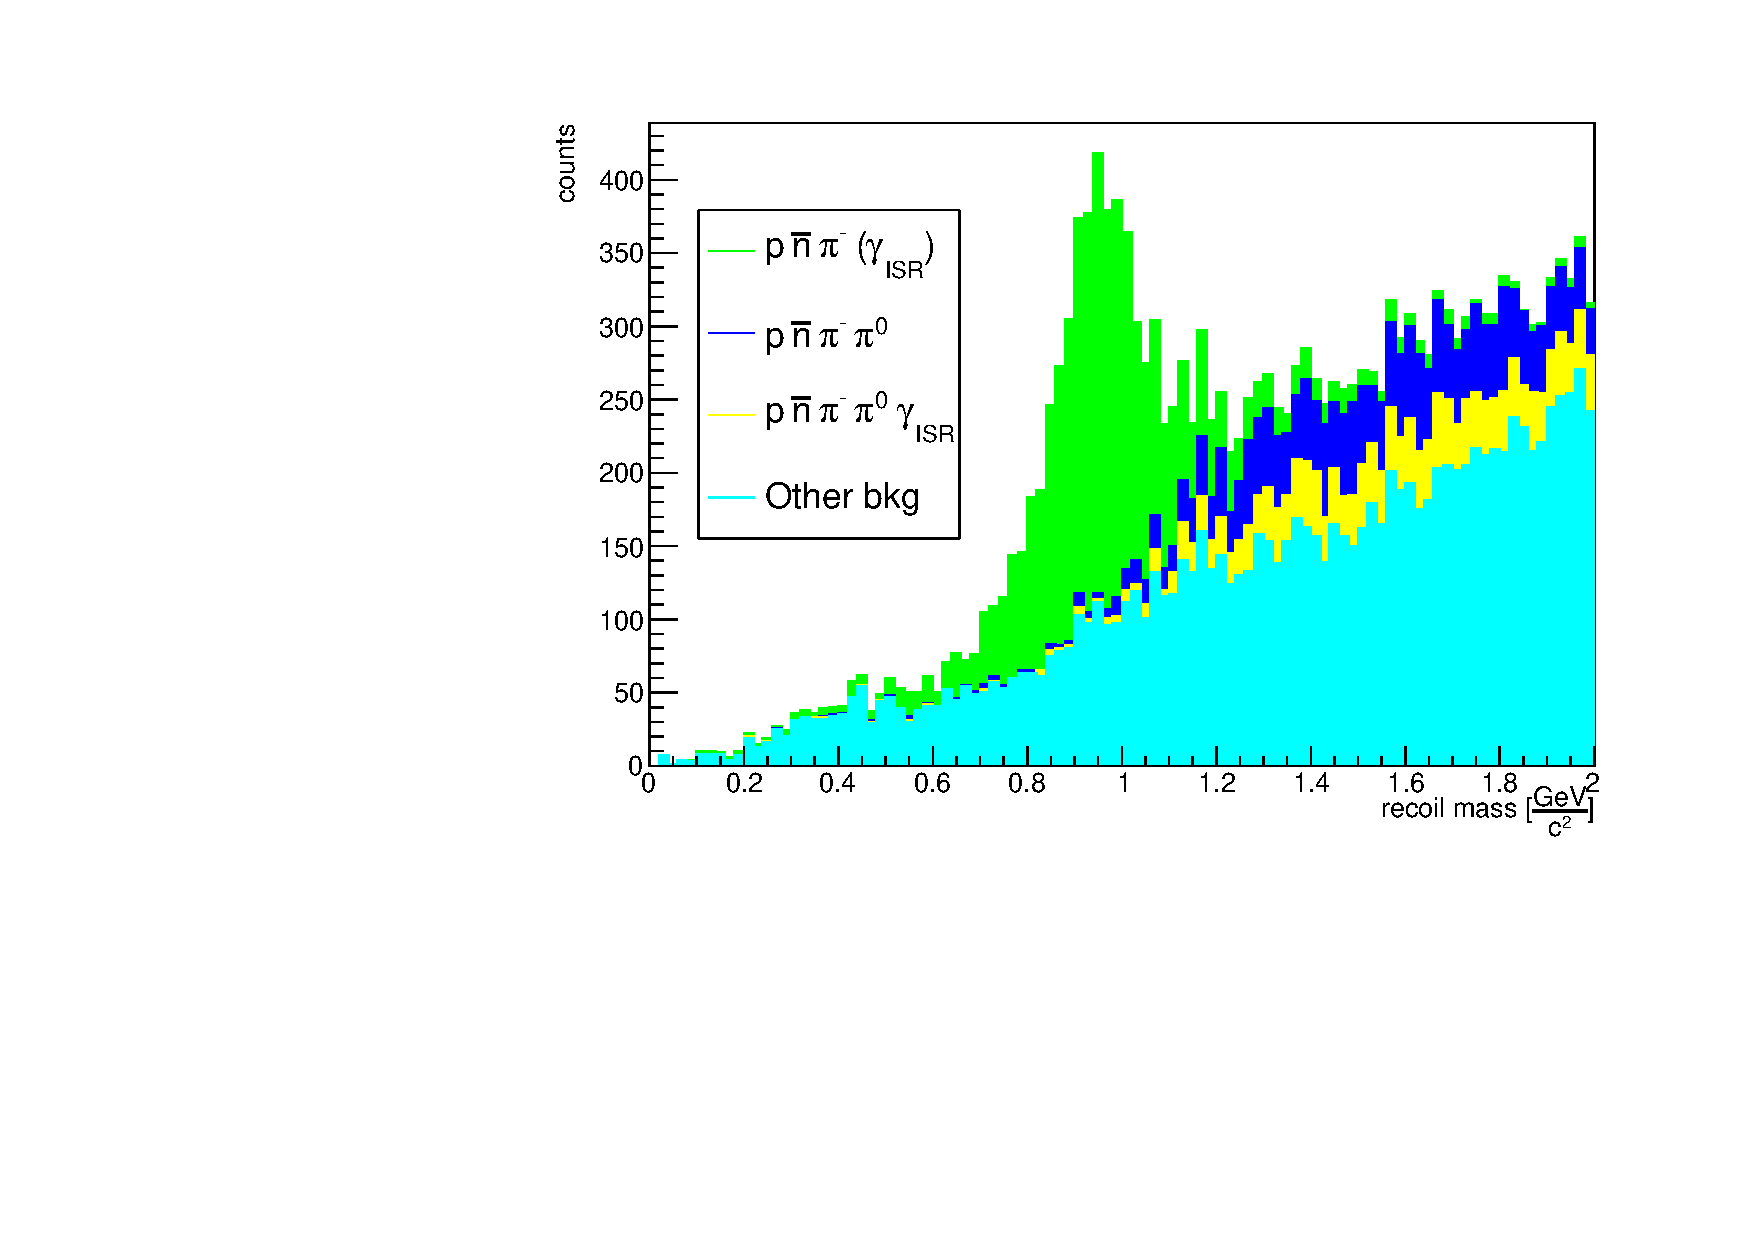
\includegraphics[width=0.90\textwidth]{nbar_cocktail/images/recoilM_comps_nog_020_0+3}
    \caption{$p, \pi^-$ recoil mass distribution in $u\bar{u}$ Monte Carlo cocktail, displaying each stacked component contribution, NO ISR case.}
    \label{fig:mRecComps_nog_020_0+3}
\end{figure}

The contributions from the remaining channels represent a flat background without discernible structures.
$\\$
To further suppress the background, a tighter $\alpha$ cut can be studied. In the next subsection, the performance of the metrics and their usage are investigated in order to find the most appropriate cut in $\alpha$.

\subsubsection{Performance metrics study on $\alpha$ cut}
In general, a \textbf{performance metric} quantifies how a classification process is optimized based on a specific parameter, which could, for example, be represented by a threshold.
$\\$
In this specific HEP context, a performance metric quantifies how well the selection cuts distinguish the signal from the background. In this analysis, the signal can be assumed to be the channel with  $\pi^- \bar{n} p (\gamma_{ISR})$ in the final state, while the background is represented by all the other channels.
$\\$
It could be useful to investigate whether a stricter cut on the $\alpha$ angle -defined as the three-dimensional angle between the recoil system and the neutral cluster associated with the anti-neutron candidate- could improve the signal selection over the background.
$\\$
To address this kind of analysis, performance metrics such as the \textbf{Figure of Merit} (FOM), the Signal Efficiency ($\epsilon_{sig}$), the Background Efficiency ($\epsilon_{bkg}$) and the \textbf{purity} can be employed. These are defined as follow:
\begin{itemize}
\item FOM = $\frac{SIGNAL(\alpha)}{\sqrt{SIGNAL(\alpha) + BACKGROUND(\alpha)}}$,
\item $ \epsilon_{sig}  = \frac{SIGNAL(\alpha)}{SIGNAL(\alpha = 0.20 \ rad)}$,
\item $ \epsilon_{bkg}  =  \frac{BACKGROUND(\alpha)}{BACKGROUND(\alpha = 0.20 \ rad)}$,
\item Purity $= \frac{SIGNAL(\alpha)}{SIGNAL (\alpha)+ BACKGROUND(\alpha)}$,
\end{itemize}
where
\begin{itemize}
 \item SIGNAL($\alpha$) is defined by the number of entries from the signal channel, depending on $\alpha$.
 \item BACKGROUND($\alpha$) is defined by the number of entries from the other channels within the signal region, depending on $\alpha$.
 \end{itemize}
SIGNAL($\alpha$) + BACKGROUND ($\alpha$) = TOTAL($\alpha$), the total  amount of entries.
$\\$
Assuming the signal region corresponds to the interval $[0.8, 1.2]$ GeV, the FOM characterizes the statistical significance of the applied threshold, namely the selected cut on $\alpha$. The higher the FOM, the more signal is selected over the background (the figure is maximized). For each possible cut value of $\alpha$, the Figure of Merit (FOM) is computed and the cut corresponding to the maximum FOM (or to a stable plateau) is selected. A higher FOM indicates a better trade-off between signal efficiency and background rejection, so the selection is optimized when the FOM is maximized. The obtained FOM is shown in Fig.~\ref{fig:fom_alpha020}.
\begin{figure}[h]
    \centering
    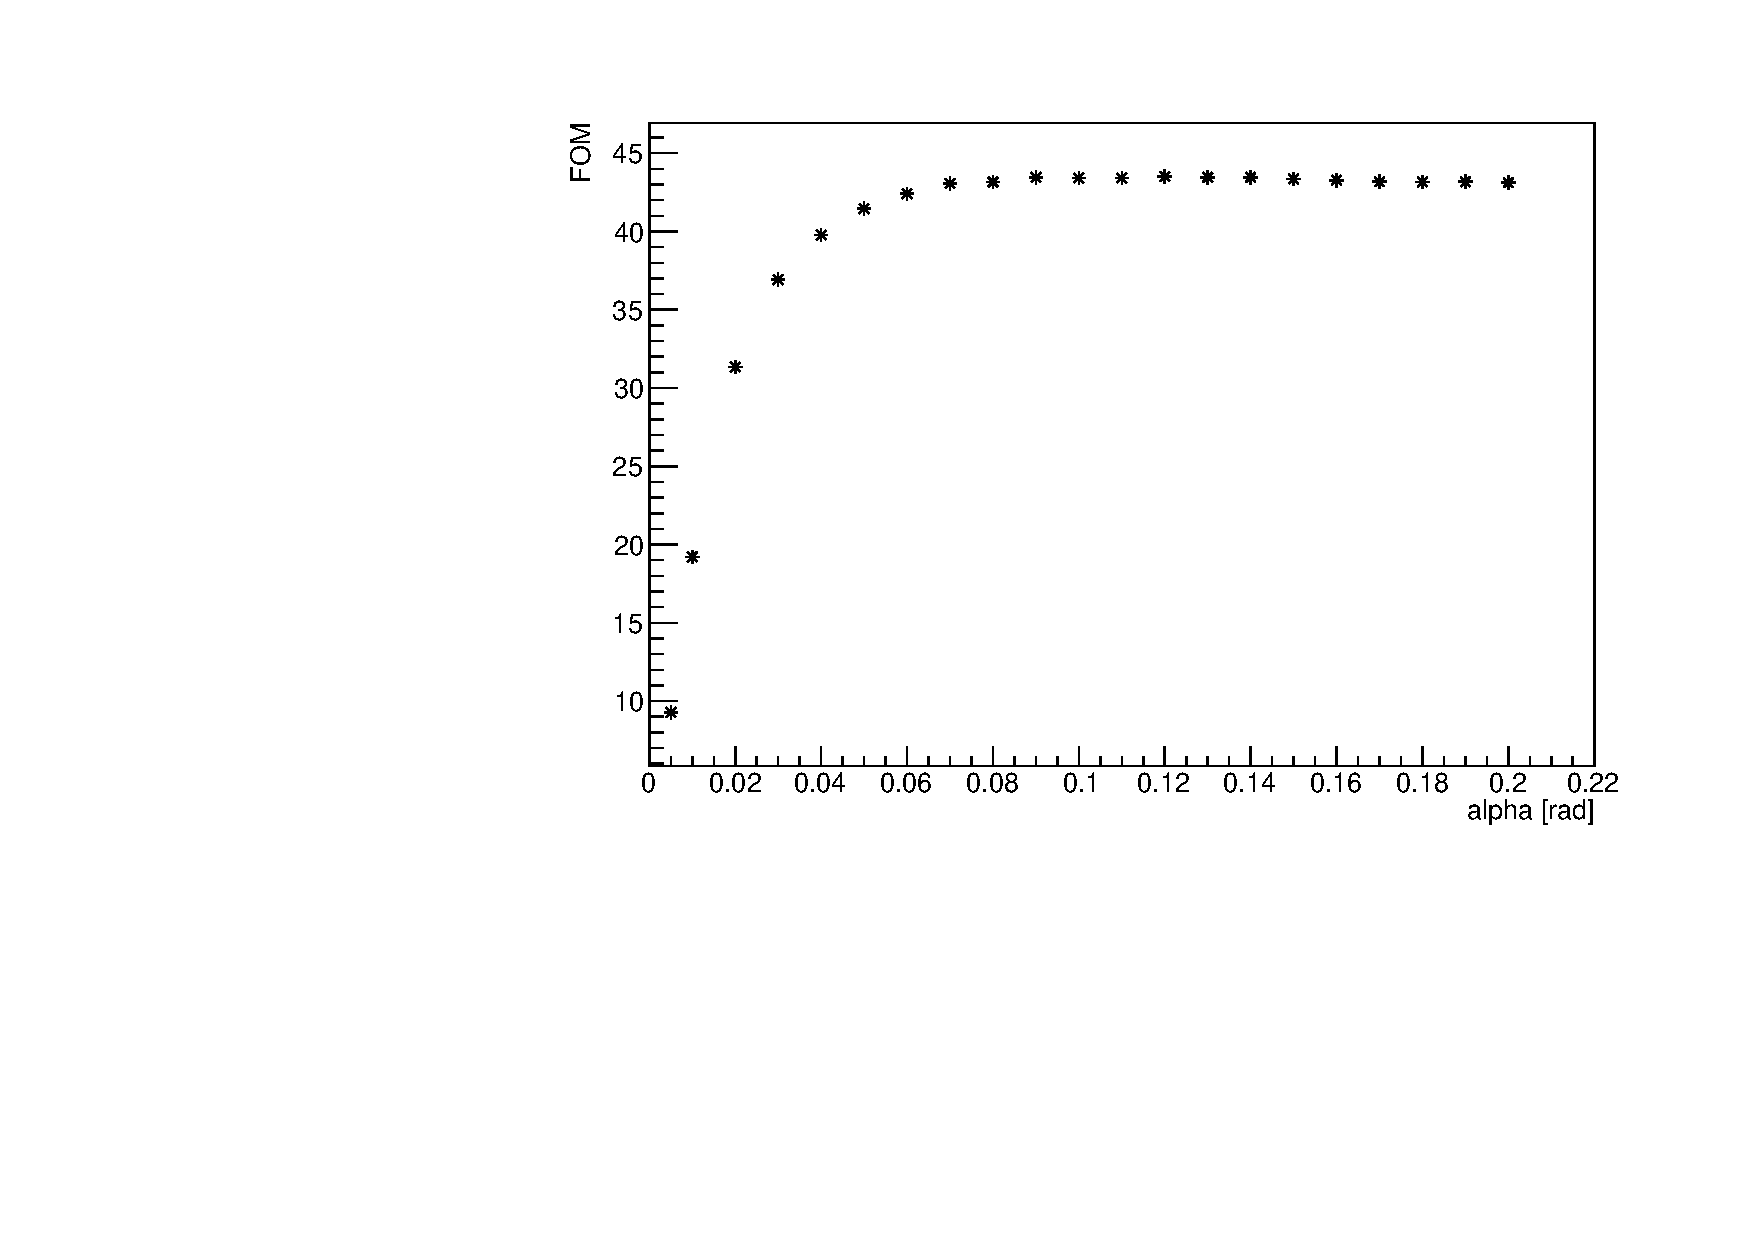
\includegraphics[width=0.70\textwidth]{nbar_cocktail/images/fom_alpha}
    \caption{Figure of Merit (FOM) versus $\alpha$ angle for the $u\bar{u}$ cocktail.}
    \label{fig:fom_alpha020}
\end{figure}
$\\$
One $\alpha$ value corresponding to the plateau can be chosen in order to maximize the FOM. The value $\alpha < 0.1$ rad ($\sim 5.73^\circ$) is therefore chosen, corresponding to FOM = 43.4185
$\\$
Furthermore, the signal efficiency $\epsilon_{sig}$ and the background efficiency $\epsilon_{bkg}$ performance metrics can be adopted to study the Receiver Operating Characteristic (ROC), a curve that shows how well a binary classifier distinguishes signal from background as the decision threshold ($\alpha$ cut) is varied.
Each point on the curve corresponds to a different threshold (a cut on the $\alpha$ angle). The Area Under the ROC Curve (AUC/ROC-AUC) is a single number summarizing the overall performance: 1.0 indicates perfect discrimination, while 0.5 corresponds to no better performance than random. The obtained ROC is shown in Fig.~\ref{fig:roc_alpha020}.
\begin{figure}[H]
    \centering
    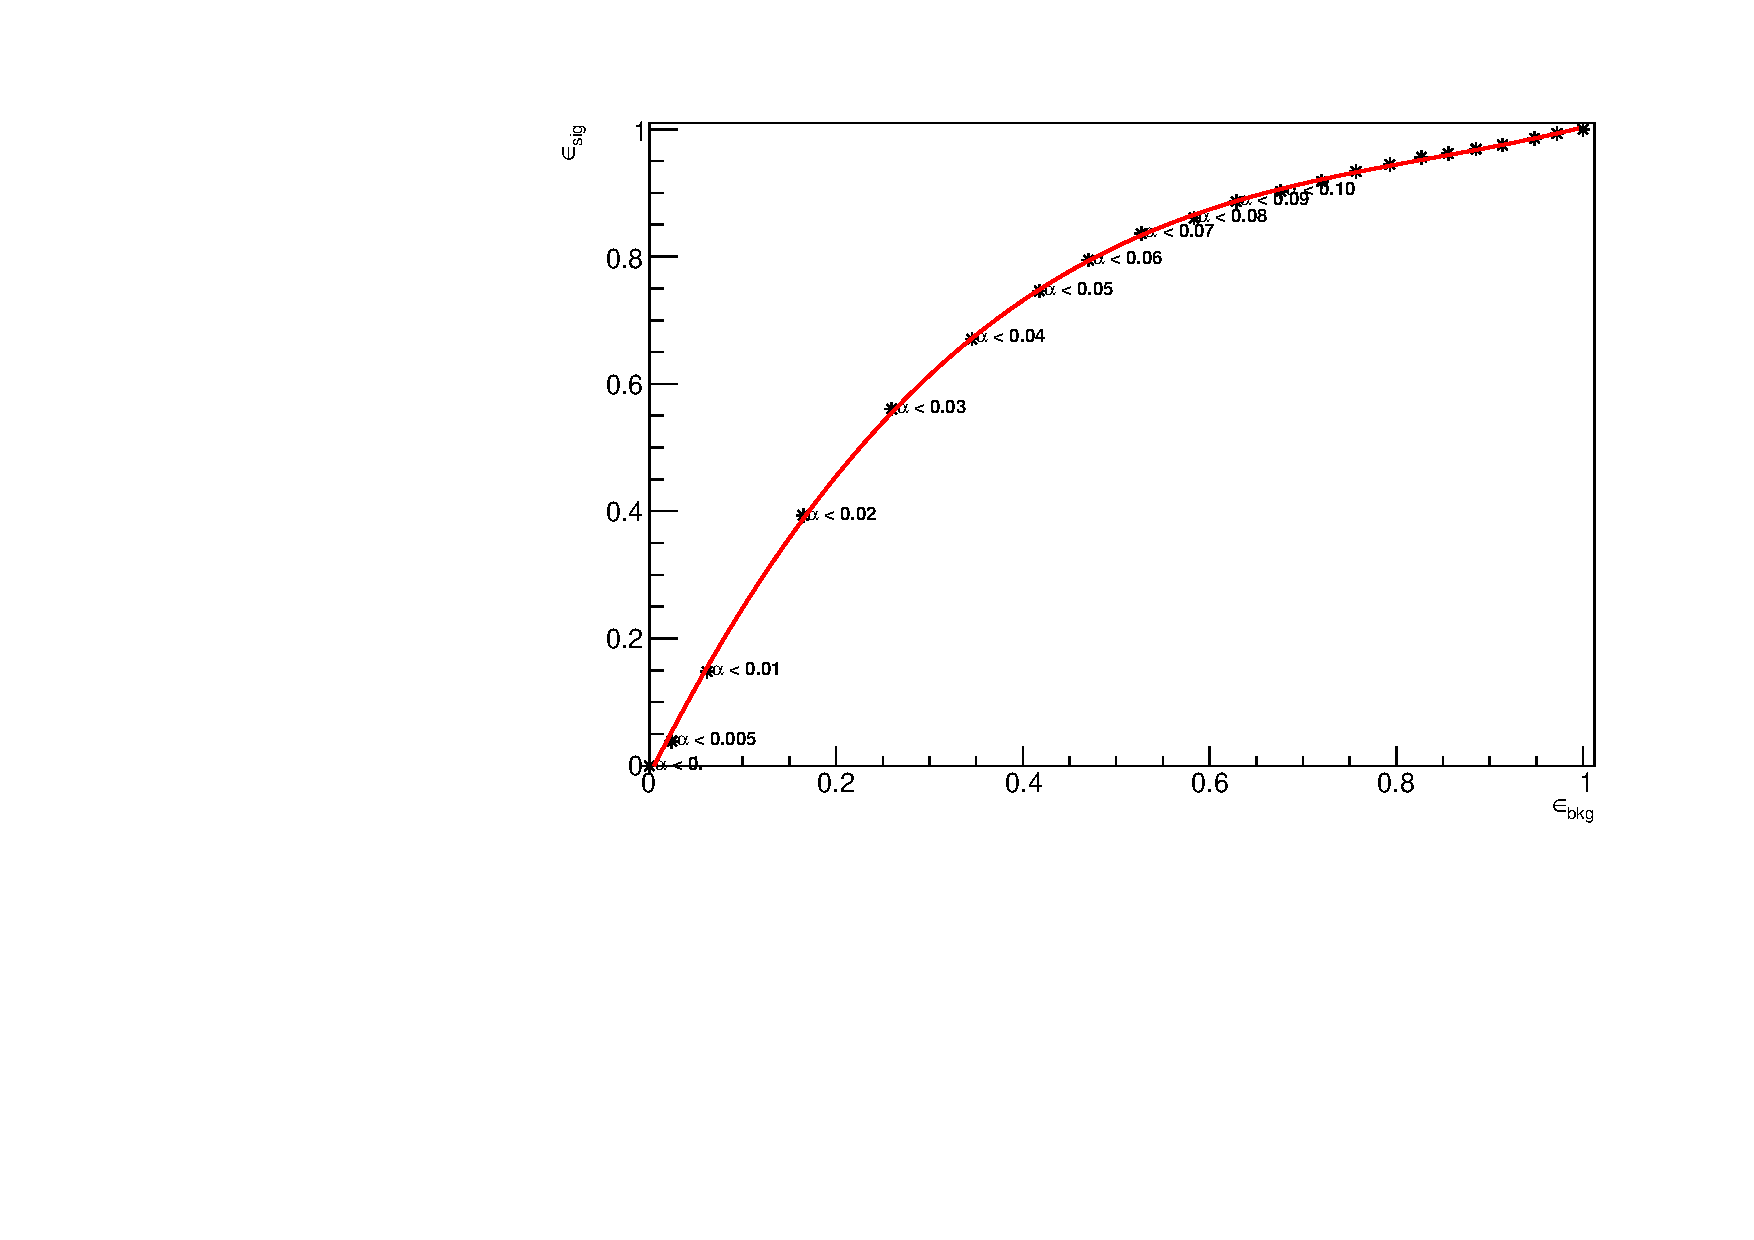
\includegraphics[width=0.70\textwidth]{nbar_cocktail/images/roc_alpha_true}
    \caption{Receiver Operating Characteristic (ROC) curve constructed from the signal efficiency ($\epsilon_{sig}$) and the Background Efficiency ($\epsilon_{bkg}$) for the $u\bar{u}$ Monte Carlo cocktail. where each point corresponds to a different cut value on the $\alpha$ angle. For clarity, the labels are shown only for $\alpha < 0.10$ rad.}
    \label{fig:roc_alpha020}
\end{figure}

The Receiver Operating Characteristic (ROC) curve for the $\alpha$ angle cut yields an area under the curve (AUC) of $0.71$, indicating good discrimination power between signal and background.
$\\$
Therefore, the obtained performance metrics for $\alpha < 0.1$ rad are:
\begin{center}
$FOM = 43.4185$, $\epsilon_{sig}= 90\%$, $\epsilon_{bkg}= 68\%$,  $Purity = 63\%$
\end{center}
The obtained $\epsilon_{sig}$ vs $Purity$ is shown in Fig.~\ref{fig:eff_alpha020}.
\begin{figure}[H]
    \centering
    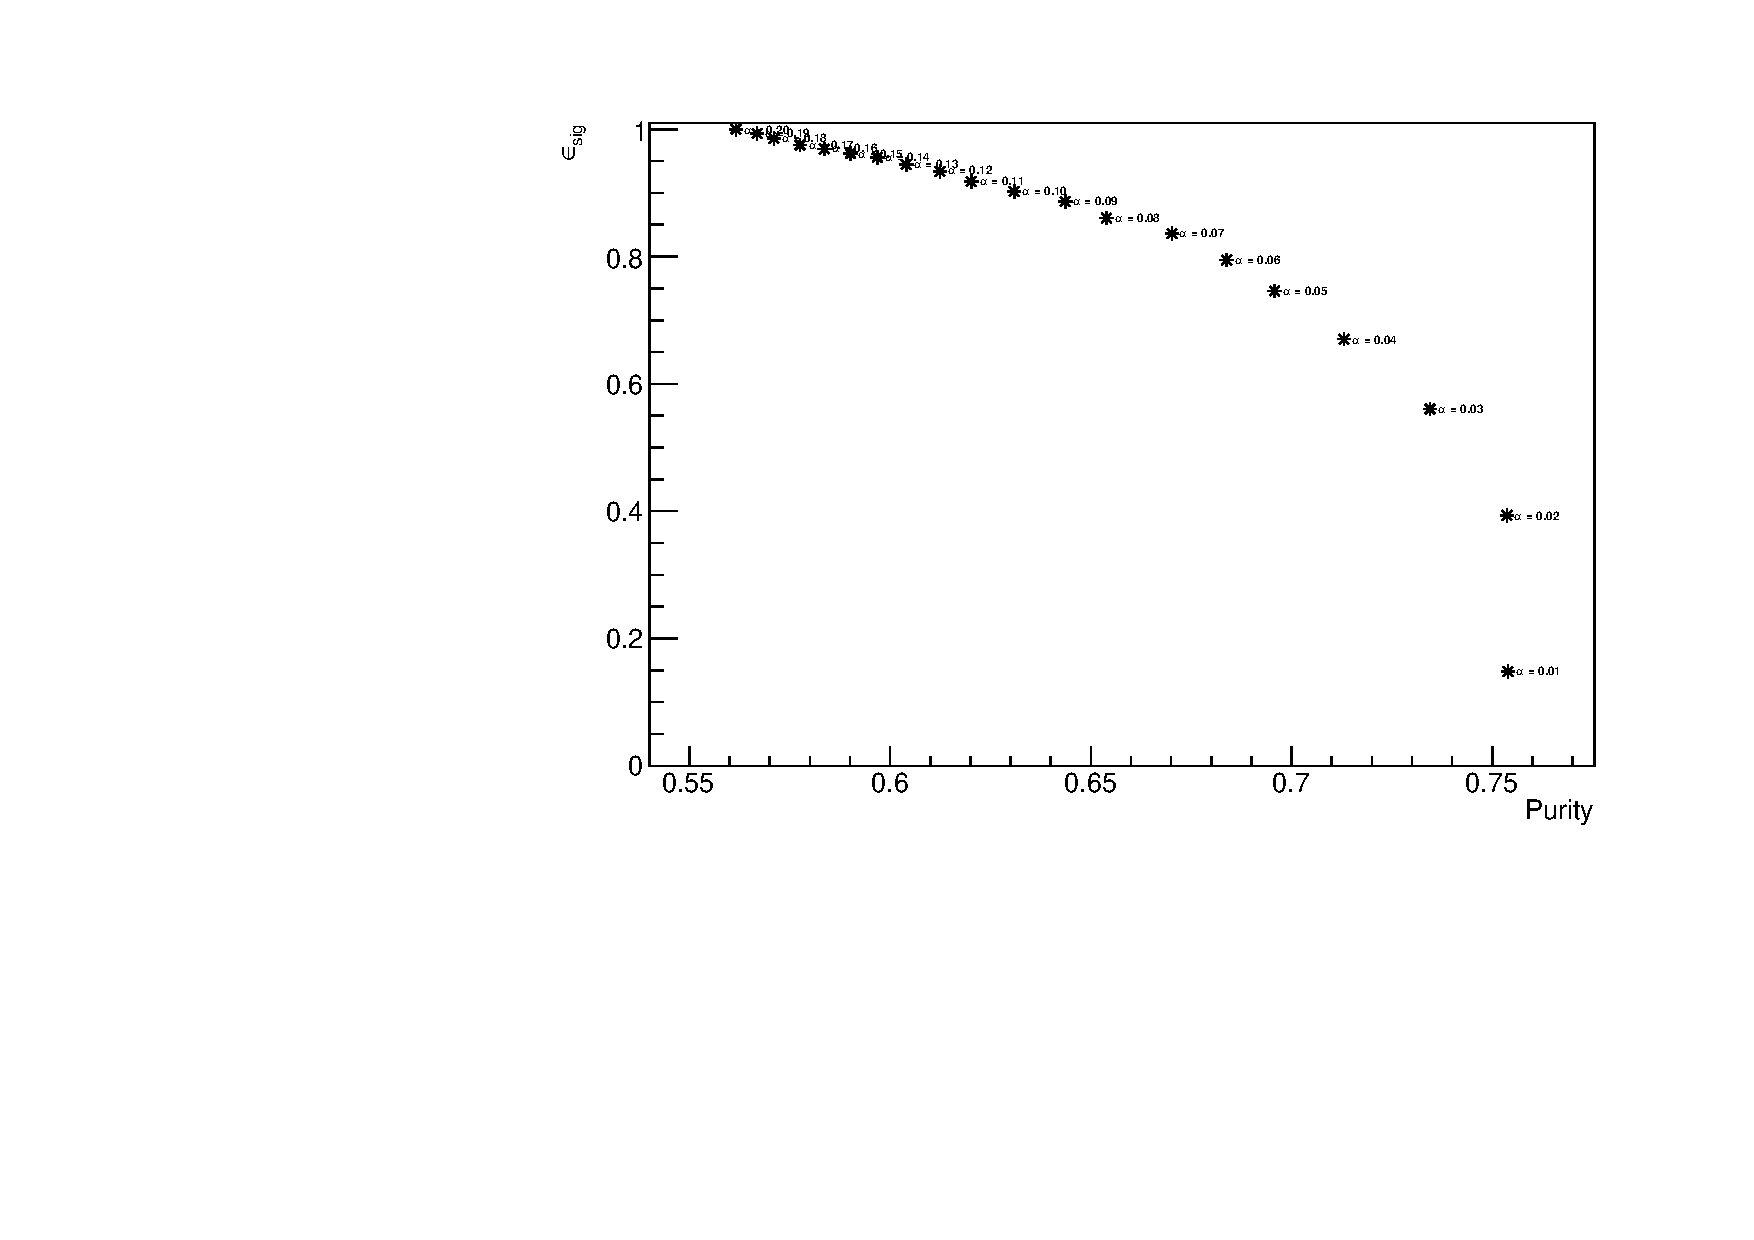
\includegraphics[width=0.70\textwidth]{nbar_cocktail/images/eff_alpha}
    \caption{ $\epsilon_{sig}$ vs $Purity$ curve for the $u\bar{u}$ Monte Carlo cocktail.}
    \label{fig:eff_alpha020}
\end{figure}
Following the optimization described, the recoil mass channel components distribution can now be analyzed using the cut $\alpha < 0.10$ rad.
$\\$
The obtained stacked component to the recoil mass are shown in figure ~\ref{fig:mRecComps_nog_010}.
\begin{figure}[h]
    \centering
    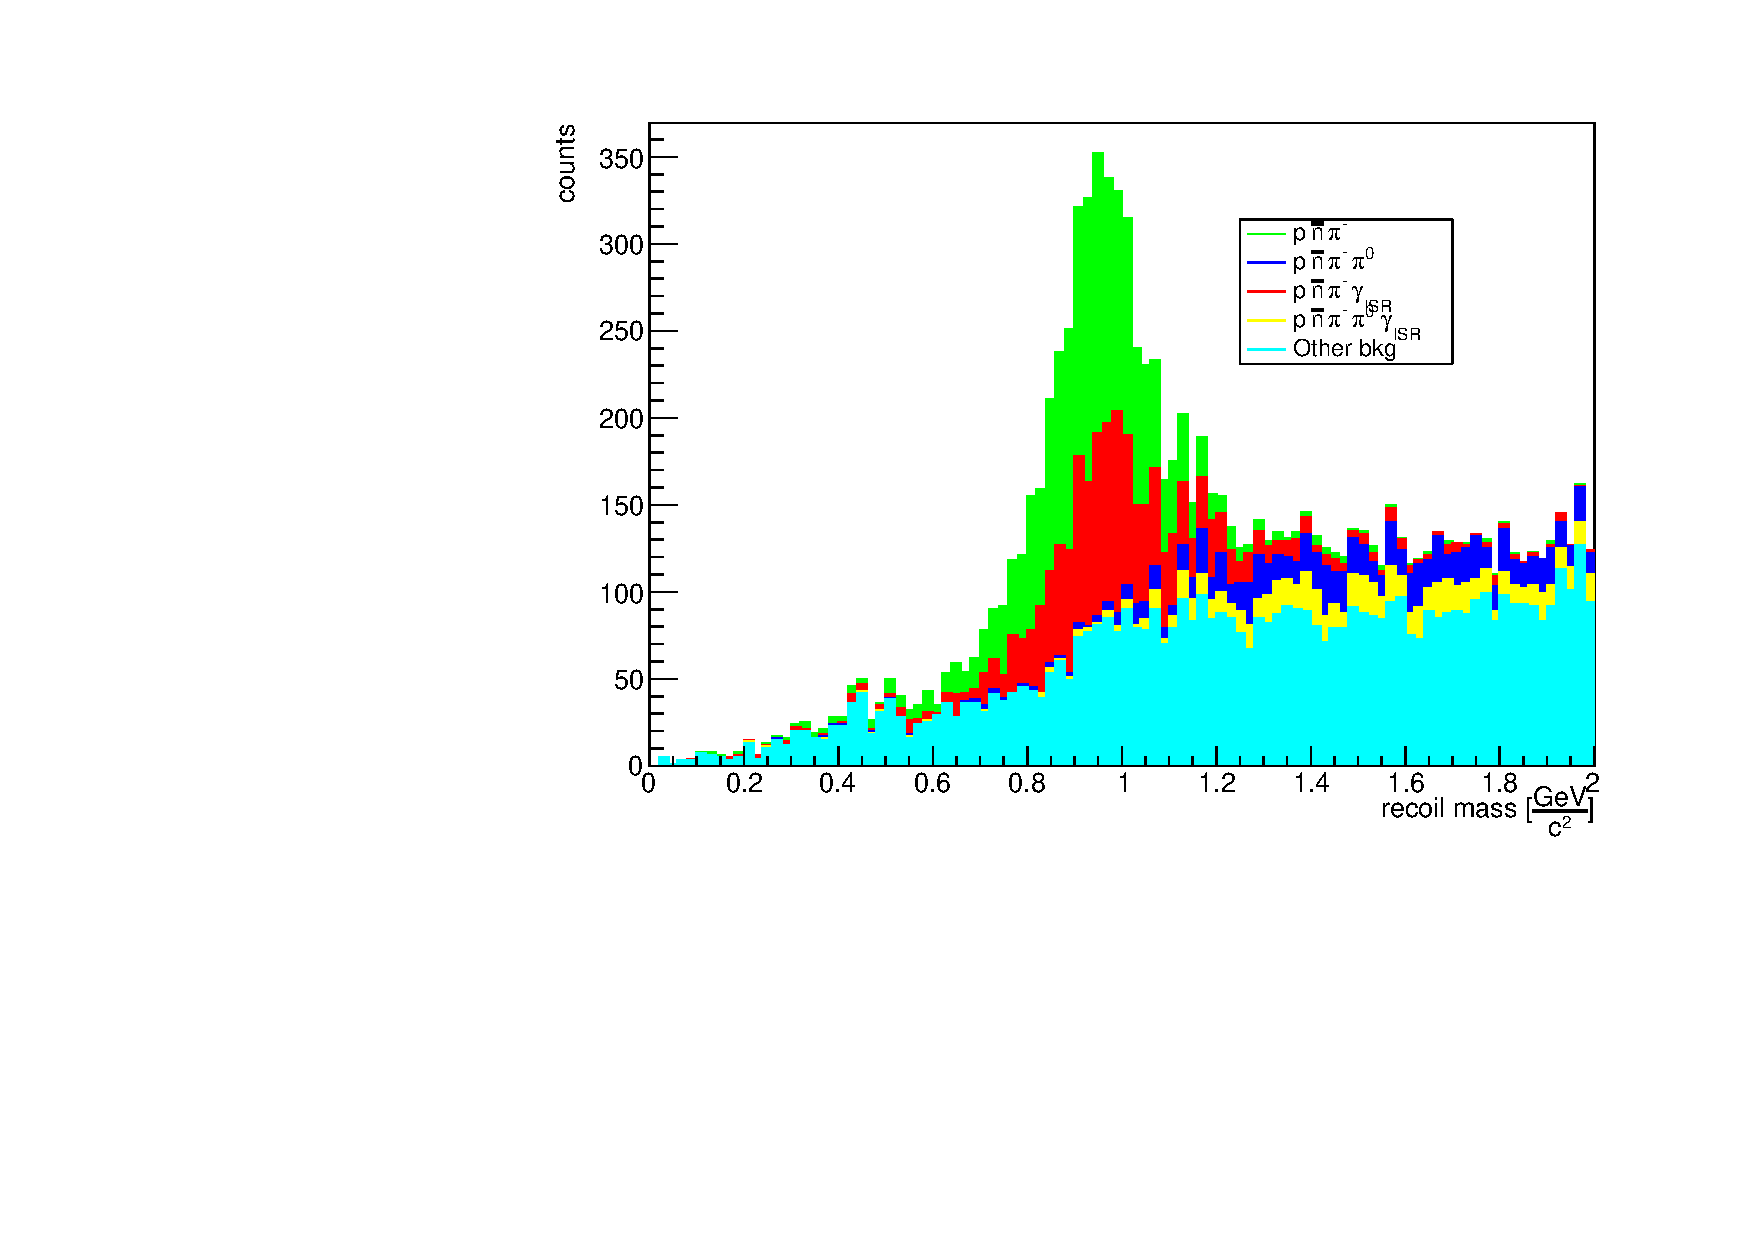
\includegraphics[width=0.7\textwidth]{nbar_cocktail/images/recoilM_comps_nog_010}
    \caption{$p, \pi^-$ recoil mass distribution in $u\bar{u}$ Monte Carlo cocktail, displaying each stacked component contribution, NO ISR case. $\alpha<$ 10 rad cut is applied.}
    \label{fig:mRecComps_nog_010}
\end{figure}

As expected, the signal is more prominent relative to the background than in the previous case. Background components containing $\pi^0$ peak outside the signal region $[0.8,1.2]$ GeV on the right side, while other sources exhibit a lower, flat distribution across the recoil mass spectrum.
$\\$
The first 5 channels of $u\bar{u}$ TopoAna output with the $\alpha<$ 10 rad cut is shown in ~\ref{fig:topo_nog_010_uubar}.
\begin{figure}[h]
    \centering
    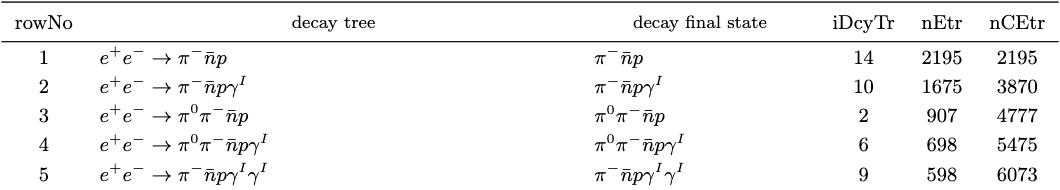
\includegraphics[width=1\textwidth]{nbar_cocktail/images/topo_uubar_010}
    \caption{Top 5 channels from the TopoAna output for the $u\bar{u}$ Monte Carlo cocktails.}
    \label{fig:topo_nog_010_uubar}
\end{figure}

After applying the $\alpha < 0.10$ rad cut, the dominant contribution remains from the signal channel $p \pi^- \bar{n}$, now immediately followed by $p \pi^- \bar{n} \gamma_{\text{ISR}}$. As discussed, both contributions can be identified as signal since they fall within the signal region $[0.8,1.2]$ GeV.

\subsection{$q\bar{q}$ cocktail production (NO ISR case)}
In order to fully characterize the Monte Carlo simulation, all $q\bar{q}$ continuum components must be studied. The Run 1 Monte Carlo productions for $u\bar{u}$, $d\bar{d}$, $s\bar{s}$, and $c\bar{c}$ are therefore analyzed. Each of them corresponds to an integrated luminosity of $\sim 1429.23 \ fb^{-1}$ of data.
$\\$
For a cleaner comparison between the signal channel and background components, the TopoAna output can be consulted in Fig.~\ref{fig:topo_nog_010_qqbar}.
\begin{figure}[H]
    \centering
    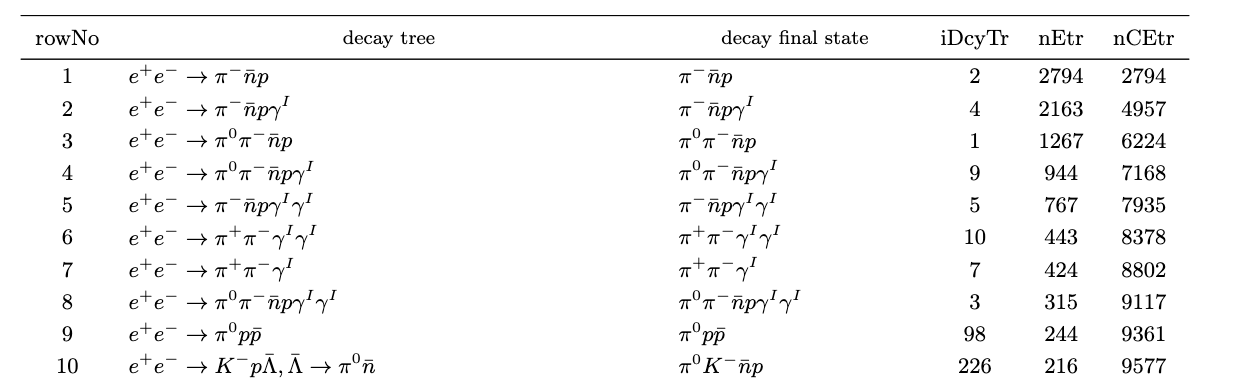
\includegraphics[width=1\textwidth]{nbar_cocktail/images/topoana_nog_010_qqbar}
    \caption{First 10 channels of the TopoAna output in $q\bar{q}$ Monte Carlo cocktail, showing the different channel contributes.}
    \label{fig:topo_nog_010_qqbar}
\end{figure}
The TopoAna output reveals that the dominant contribution is from the signal channel $p \pi^- \bar{n}$ in the $q\bar{q}$ continuum. A secondary contribution comes from $p \pi^- \bar{n} \gamma_{ISR}$, which could be treated as signal despite the $\gamma_{\text{ISR}}$ not being explicitly reconstructed.The next contribution comes from $p \pi^- \bar{n} \pi^0$ in the final state. The fourth contribution is due to $p \pi^- \bar{n} \pi^0 \gamma_{\text{ISR}}$, and so on. The situation is very similar to that observed in the $u\bar{u}$ case.
$\\$
It would be interesting to discuss the individual TopoAna outputs separately for the $u\bar{u}$, $d\bar{d}$, $s\bar{s}$, and $c\bar{c}$ samples. The first 5 contributes for each sample are shown in ~\ref{fig:topo_nog_010_qqbar_singles}.
\begin{figure}[h]
    \centering
    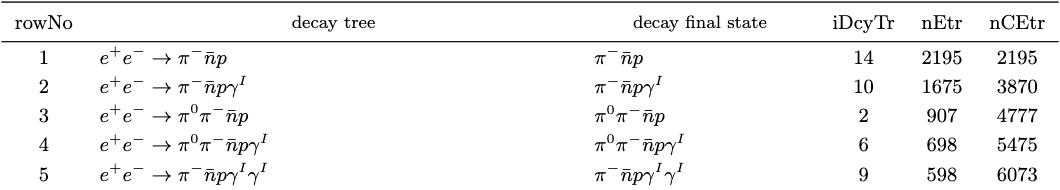
\includegraphics[width=1\textwidth]{nbar_cocktail/images/topo_uubar_010}
    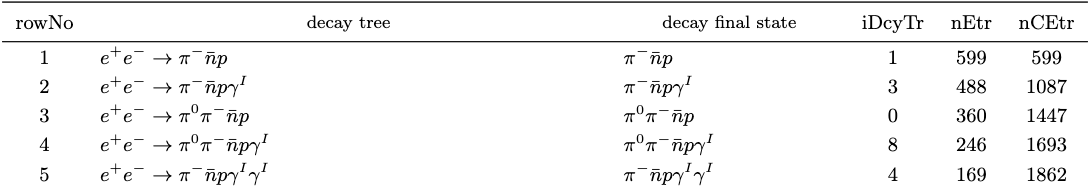
\includegraphics[width=1\textwidth]{nbar_cocktail/images/topo_ddbar_010}
    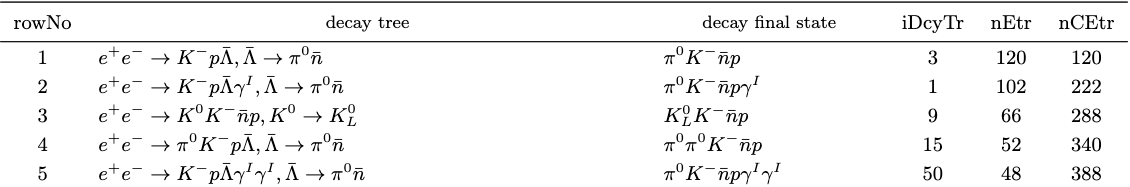
\includegraphics[width=1\textwidth]{nbar_cocktail/images/topo_ssbar_010}
    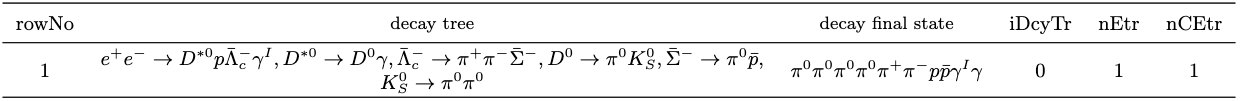
\includegraphics[width=1\textwidth]{nbar_cocktail/images/topo_ccbar_010}
    \caption{Top 5 channels from the TopoAna output respectively for the $u\bar{u}$, $d\bar{d}$, $s\bar{s}$, and $c\bar{c}$ Monte Carlo cocktails (from top to bottom). The \texttt{iDcyTr} index values may differ across samples since each TopoAna output is produced independently from its corresponding ROOT ntuples.}
    \label{fig:topo_nog_010_qqbar_singles}
\end{figure}






